\chapter{Markovketten}

\input{chapters/markovketten/Vorbermerkungen.tex}

\section{Stochastische Prozesse}
\begin{definition}Ein stochastischer Prozess ist 
eine Familie $(X_t,t\in T)$ von Zufallsvariablen. Die Indexmenge $T$
wird Parameterraum genannt und soll eine Teilmenge der reellen Zahlen sein.
Der Wertebereich $M_X$ von $X_t$ heißt Zustandsraum oder Phasenraum.
Wenn $T$ endlich oder abzählbar (etwa $\mathbb N$) 
ist, sprechen wir von einem Prozess in
diskreter Zeit, wenn $T$ ein ganzes (endliches oder unendliches) Intervall
ist, von einem Prozess in stetiger Zeit, 
\end{definition}
Stochastische Prozesse in diskreter Zeit sind einfach Folgen von
 Zufallsvariablen. Der Unterschied zu unseren früheren Überlegungen besteht 
darin, dass wir nicht mehr annehmen, dass die einzelnen Zufallsvariablen
unabhängig sind. Wir müssen also die Abhängigkeiten zwischen den einzelnen
Zufallsvariablen festlegen, das heißt, wir müssen gewisse Annahmen über
die gemeinsame Verteilung von $(X_{t_1},\dots,X_{t_n})$ mit 
$t_1<\dots<t_n$ treffen (Ein berühmter Satz von Kolmogorov besagt, dass
durch die Angabe dieser ``endlichdimensionalen Randverteilungen'' ein
stochastischer Prozess festgelegt wird). 
Einige Möglichkeiten zählen wir jetzt auf:
\begin{definition}
Der Prozess $(X_t, t\in T)$ heißt Prozess mit unabhängigen Zuwächsen,
wenn für $t_1<t_2<\dots>t_n$ die Zufallsvariablen
\[X(t_1), X(t_2)-X(t_1), X(t_3)-X(t_2),\dots, X(t_n)-X(t_{n-1})\]
unabhängig sind.
\end{definition}
Hier verwenden wir die Notation $X(t)$ für $X_t$, damit die Indizes nicht
zu sehr überladen werden. 
Prozesse mit unabhängigen Zuwächsen in diskreter Zeit sind einfach
Summen von unabhängigen Zufallsvariablen, wie wir sie im letzten Kapitel
untersucht haben.
\begin{definition}
Der Prozess $X(t)$ heißt Markovprozess, wenn für
wenn für $t_1<t_2<\dots>t_n$ 
\[\mathbb P(X(t_n)\le x_n|X(t_1)=x_1,\dots,X(t_{n-1})=x_{n-1})=
\mathbb P(X(t_n)\le x_n|X(t_{n-1})=x_{n-1}).\]
\end{definition}
Die Zukunft hängt also von der Vergangenheit nur über den letzten Wert
$X(t_{n-1})$ ab. Ein Beispiel für Markovprozesse sind Prozesse mit
unabhängigen Zuwächsen.
\begin{definition}
Der Prozess $X_t,t\in T$ heißt stationär, wenn
wenn für $t_1<t_2<\dots>t_n$ und $h>0$
die gemeinsame Verteilung von $(X(t_1),\dots,X(t_n))$
mit der von $(X(t_1+h),\dots,X(t_n+h))$ übereinstimmt.
\end{definition}
\section{Markovketten in diskreter Zeit}
\subsection{Übergangswahrscheinlichkeiten}
\label{sec:uebergangswahrscheinlichkeit}
\index{"Ubergangswahrscheinlichkeit@Übergangswahrscheinlichkeit}
%TODO
Markovprozesse mit diskretem Zustandsraum nennen wir Markovketten. Wir 
können noch zwischen Markovketten in diskreter und in stetiger Zeit
unterscheiden. Die Diskussion von Markovketten in stetiger Zeit
werden wir auf später verschieben. In beiden Fällen kann man die
diskrete Verteilung der einzelnen Zufallsvariablen durch ihre Wahrscheinlichkeitsfunktion beschreiben, deshalb erhält die Markoveigenschaft die besonders einfache Form
\[\mathbb P(X_n= x_n|X_1=x_1,\dots,X_n=x_n)=
\mathbb P(X_n=x_n|X_{n-1}=x_{n-1}).\]
Die Wahrscheinlichkeiten
\[\mathbb P(X_{n+1}=j|X_n=i)\]
nennen wir die Übergangswahrscheinlichkeiten der Markovkette. Wenn diese
nicht von $n$ abhängen, sprechen wir von einer homogenen Markovkette und
setzen
\[p_{ij}=\mathbb P(X_{n+1}=j|X_n=i)\]

\begin{definition}
Die Wahrscheinlichkeiten
\[p_{ij}(t)=\mathbb P(X_{n+t}=j|X_n=i)\]
nennen wir die \textbf{$t$-stufigen Übergangswahrscheinlichkeiten}. 
Aus dem Satz von der vollständigen Wahrscheinlichkeit erhalten wir
die \textbf{Chapman-Kolmogorov Gleichungen}\index{Chapman-Kolmogorov Gleichungen}\index{Kolmogorov-Chapman Gleichungen|see{Chapman-Kolmogorov Gleichungen}} 
\end{definition}
%TODO: nicht als eigenen satz oder definition oder so???
\[p_{ij}(s+t)=\sum_{k\in M_X}p_{ik}(s)p_{kj}(t).\]
in Matrixnotation mit
\[P(t)=(p_{ij}(t))_{M_X\times M_X}\]
lauten die Chapman-Kolmogorov
Gleichungen
\[P(t+s)=P(t)P(s),\]
und mit $P=P(1)$
\[P(t)=P^t.\]
Wir nennen $P$ die \textbf{Übergangsmatrix} und $P(t)$ die \textbf{t-stufige Übergangsmatrix}.
\index{"Ubergangsmatrix@Übergangsmatrix}\index{"Ubergangsmatrix@Übergangsmatrix!t-stufige}

Wir setzen zusätzlich $p_i(t)=\mathbb P(X_t=i)$ und $p(t)=(p_i(t),i\in M_X)$
(als Zeilenvektor). Wieder mit dem Satz von der vollständigen Wahrscheinlichkeit erhalten wir
\[p(t)=p(0)P^t.\]
Wie man am besten Matrixpotenzen berechnet, siehe Anhang \ref{sec:matrixpotenz}.
Durch $p(0)$ und $P$ werden alle endlichdimensionalen Verteilungen festgelegt.

In Hinkunft verwenden wir zur Abkürzung die Notationen
\[\mathbb P_i(A)=\mathbb P(A|X_0=i)\]
und
\[\mathbb E_i(Y)=\mathbb E(Y|X_0=i).\]
\subsection{Klasseneigenschaften}
\label{sec:klasseneigenschaften}
Wir definieren
\begin{definition}
    \label{def:nachfolger}\label{def:verbunden}\label{def:kommunizierend}
    \index{Nachfolger}
Der Zustand $j$ heißt \textbf{Nachfolger} von $i$ ($i\rightarrow j$), wenn es ein
$t\ge 0$ gibt, sodass $p_{ij}(t)>0$.

Wenn sowohl $i\rightarrow j$ als auch $j\rightarrow i$ gilt, dann heißen
$i$ und $j$ \textbf{verbunden} oder \textbf{kommunizierend}.\index{verbunden}\index{kommunizierend}
\end{definition}

Das Kommunizieren ist eine Äquivalenzrelation, wir können daher 
den Phasenraum in die Äquivalenzklassen zerlegen, die wir Rekurrenzklassen
oder kurz Klassen nennen. Gibt es nur eine Klasse (wenn also alle
Zustände miteinander kommunizieren), heißt die Markovkette \textbf{irreduzibel}\index{irreduzibel}.
\index{absorbierender Zustand}\index{Zustand, absorbierend|see{absorbierender Zustand}}
Ein Zustand mit $p_{ii}=1$ heißt \textbf{absorbierender Zustand}. Ein solcher Zustand
ist offensichtlich eine Klasse für sich (no pun intended).
\begin{definition}
    \label{def:klasseneigenschaft}
Eine Eigenschaft heißt \textbf{Klasseneigenschaft}\index{Klasseneigenschaft}, wenn sie entweder für alle
Zustände einer Klasse oder für  keinen gilt.
\end{definition}

Ein einfaches Beispiel einer Klasseneigenschaft ist die Periode:
\begin{definition}
    \label{def:periode}\index{Periode}
Die \textbf{Periode} eines Zustandes ist
\[d(i)=\mathrm{ggT}\{t\ge 0:p_{ii}(t)>0\}.\]

Sie definiert also den kleinsten möglichen Weg, um von Zustand $i$ wieder zum Zustand $i$ zurückzukehren.
\end{definition}
Etwas spannender ist die \textbf{Rekurrenz}\index{Rekurrenz}: dazu definieren wir zuerst
\[\tau_i=\inf\{t>0:X_t=i\},\]
die \textbf{Übergangszeit}\index{"Ubergangszeit@Übergangszeit} bzw.\ \textbf{Rückkehrzeit}\index{R"uckkehrzeit@Rückkehrzeit} (je nachdem, ob $X_0\neq i$ ist
oder nicht) nach $i$,
und
\[\nu_i=\#\{t>0:X_t=i\},\]
die Anzahl der Besuche in $i$.

\begin{satz}
Die folgenden Bedingungen sind äquivalent:
\begin{enumerate}
\item $\mathbb P_i(\tau_i<\infty)=1$,
\item $\mathbb P_i(\nu_i=\infty)=1$,
\item $\mathbb E_i(\nu_i)=\infty$,
\item $\sum_tp_{ii}(t)=\infty$.
\end{enumerate}
Wenn diese Bedingungen erfüllt sind, dann heißt $i$ rekurrent, sonst
transient. Rekurrenz und Transienz sind Klasseneigenschaften.
\end{satz}

Bei der Rekurrenz kann man weiter unterscheiden:
\begin{definition}
$i$ sei ein rekurrenter Zustand. Wenn 
\[\mathbb E_i(\tau_i)<\infty\]
gilt, dann heißt $i$ \textbf{positiv rekurrent}, sonst \textbf{nullrekurrent}.\index{Rekurrenz!positiv-|see{positiv Rekurrent}}\index{Rekurrenz!null-|see{Nullrekurrent}}\index{Nullrekurrent}\index{positiv Rekurrent}
\end{definition}

\begin{definition}
$(\pi_i, i\in M_X)$ heißt \textbf{stationäre Verteilung}\index{stationäre Verteilung}, wenn
\[\pi_i\ge 0,\]
\[\sum_i\pi_i=1\]
und
\[\sum_i \pi_ip_{ij}=p_j.\]

Die stationäre Verteilung ist die Verteilung, die man für die Zustände
einer Markovkette erhält, wenn man sie nach einer sehr langen Zeit betrachtet. Dann sollten die Anfangseffekte (= Anfangswahrscheinlichkeit)
nicht mehr sichtbar sein. Dazu müssen wir erst die Wahrscheinlichkeit für
einen Zustand $i$ zum Zeitpunkt $t$ berechen.
\end{definition}

\begin{satz}
Wenn $(X_n)$ irreduzibel und aperiodisch ist, dann existieren die
Grenzwerte
\[\lim_{n\to\infty}p_{ij}(t)=\pi_j={1\over \mathbb E_j(\tau_j)}.\]
Im periodischen Fall gilt
\[\pi_j=\lim_{n\to\infty}{1\over n}\sum_{t=1}^{n}p_{ij}(t).\]
Wenn $(\pi_i)$ nicht identisch verschwindet (also wenn die Kette positiv
rekurrent ist), dann ist es eine
\textbf{stationäre Verteilung}\index{stationäre Verteilung}. Umgekehrt folgt aus der Existenz
einer stationären Verteilung die positive Rekurrenz. Die positive Rekurrenz
bzw.\ Nullrekurrenz ist ebenfalls eine Klasseneigenschaft.
\end{satz}

Für einen absorbierenden Zustand $i_0$ definieren wir die 
\textbf{Absorptionswahrscheinlichkeit $a_i$}\index{Absorptionswahrscheinlichkeit} als
\[\mathbb P_i(\tau_{i_0}<\infty)=\mathbb P_i(X\mbox{wird in }i_0\mbox{ absorbiert}).\]



\begin{satz}
Die Absorptionswahrscheinlichkeiten sind die kleinste nichtnegative Lösung
des Gleichungssystems
\[a_{i_0}=1,\]
\[a_i=\sum_jp_{ij}a_j, i\neq i_0.\]
\end{satz}

Das gibt uns eine Möglichkeit, die Transienz oder Rekurrenz einer
irreduziblen Markovkette zu entscheiden. Wir wählen einen Zustand und
machen ihn zu einem absorbierenden Zustand und bestimmen für die
modifizierte Übergangsmatrix die Absorptionswahrscheinlichkeiten. Sind diese
gleich 1, ist die Kette rekurrent. 

Wir nehmen an, dass $i_0$ der einzige absorbierende Zustand ist und
alle anderen Zustände kommunizieren und die Absorptionswahrscheinlichkeiten
1 sind.
Dann erhalten wir für die mittlere Zeit bis zur Absorption (\textbf{mittlere Absorptionszeit}\index{mittlere Absorptionszeit}\index{Absorptionszeit!mittlere -|see{mittlere Absorptionszeit}})
\[m_i=\mathbb E_i(\tau_{i_0})\]
 eine ähnliche Gleichung:
\[m_{i_0}=0,
\]
\[m_i=1+\sum_jp_{ij}m_j, i\neq i_0.\]

Allgemeiner kann man eine Zufallsvariable 
$S=\sum_{t=1}^{\tau-1}x_{t,t+1}$ betrachten (d.h., wir ``sammeln'' auf
unserem Weg zur Absorption Beträge $x_{ij}$, die von dem jeweiligen
Übergang abhängen dürfen). 

Wir setzen 
\[m_i=\mathbb E_i(S)\]
und
\[v_i=\mathbb V_i(S).\]

Dann sind $m_i$ und $v_i$ die Lösungen der Gleichungen

\[m_{i_0}=0,v_i(i_0)=0,\]
\[m_i=\sum_jp_{ij}x_{ij}+\sum_jp_{ij}m_j, i\neq i_0.\]
\[v_i=\sum_jp_{ij}(x_{ij}i+m_j-m_i)^2+\sum_jp_{ij}v_j, i\neq i_0.\]

Wenn es mehrere absorbierende Zustände Zustände gibt, $A=\{i_1,\dots,i_k\}$,
dann kann man die Wahrscheinlichkeiten der Absorption  $a_i(i_j)$ in dem
absorbierenden Zustand $i_j$ oder allgemeiner in einem der Zustände in der
Menge $B\subseteq A$ ($a_i=a_i(B)$). Das gibt die Gleichungen
\[a_i=\sum_jp_{ij}a_j, i\not\in A\]
\[a_i=1, i\in B\]
\[a_i=0, i\in A\setminus B.\]

Manchmal ist es interessant (wieviel Geld werde ich haben, wenn ich nicht
bankrott gehe?), den Erwartungswert von $S$ unter der Bedingung, dass die
Absorption in einem bestimmten Zustand oder in einer bestimmten Teilmenge
der Menge der absorbierenden Zustände erfolgt. 
Da hilft es, dass $X(t)$ unter der Bedingung der Absorption in $B$
wieder eine Markovkette bildet, mit den Übergangswahrscheinlichkeiten
\[p_{ij}^B={p_{ij}a_j(B)\over a_i(B)}.\]
Mit diesen modifizierten Übergangswahrscheinlichkeiten (wobei die
absorbierenden Zustände $\not\in B$ weggelassen werden) kann man
die Gleichungen für $m_i$ $v_i$ lösen und erhält so die bedingte
Erwartung bzw.\ Varianz.




\subsection{Markov Chain Monte Carlo}


\ifdefined\uebsps
\newExercPage
\begin{uebsp}
\begin{Exercise}[label=ex:4.1]
Zwei Spieler A und B mit Kapital $a$ und $b$ spielen folgendes Spiel: In jeder Runde setzt jeder Spieler einen Einsatz 1. Dann wird eine Münze geworfen, und A gewinnt, wenn sie ''Kopf'' zeigt, sonst gewinnt B. Das Spiel ist zu Ende, wenn ein Spieler kein Kapital mehr hat. Überlegen Sie, dass $X_t$, das Kapital von A zum Zeitpunkt $t$, eine Markovkette bildet, bestimmen Sie die Übergangsmatrix und die Klassen und ihre Perioden.
\end{Exercise}
\begin{Answer}

\begin{uebsp_theory}
    Bei Markovketten 1.Ordnung hängt die Zukunft nur von der Gegenwart (dem aktuellen Zustand) ab.
\end{uebsp_theory}

\begin{description}
    \item [Die Markovkette]:\\
        \begin{tikzpicture}[->,>=stealth',shorten >=1pt,auto,node distance=0.95cm,
                    semithick]
  \tikzstyle{every state}=[fill=blue!30,draw=none,text=white,minimum size=0.35cm]

  \node[state]              (0)                                         {};
  \node[state]              (1)      [right of=0]                       {};
  \node[state]              (2)      [right of=1]                       {};
  \node[state, fill=none]   (3)      [right of=2]                       {};
  \node[state, fill=none]   (a-2)    [right of=3, node distance=0.8cm]  {};
  \node[state]              (a-1)    [right of=a-2]                     {};
  \node[state]              (a)      [right of=a-1]                     {};
  \node[state]              (a+1)    [right of=a]                       {};
  \node[state, fill=none]   (a+2)    [right of=a+1]                     {};
  \node[state, fill=none]   (a+b-3)  [right of=a+2, node distance=0.8cm]{};
  \node[state]              (a+b-2)  [right of=a+b-3]                   {};
  \node[state]              (a+b-1)  [right of=a+b-2]                   {};
  \node[state]              (a+b)    [right of=a+b-1]                   {};

  \node (desc0) [below of=0,node distance=1.6cm, align=center] {Zustand 0\\Absorbierend};
  \node (desca+b) [below of=a+b,node distance=1.6cm, align=center] {Zustand a+b\\Absorbierend};
  \node (desca) [below of=a,node distance=1.6cm, align=center] {Zustand a\\Start};

  \path (0) edge [loop above]   node {$1$} (0)
        (1) edge                node [above]{$\frac{1}{2}$} (0)
            edge [bend right]   node [below]{$\frac{1}{2}$} (2)
        (2) edge [bend right]   node [above]{$\frac{1}{2}$} (1)
            edge [bend right]   node [below]{$\frac{1}{2}$} (3)
        (3) edge [bend right]   node [above]{$\frac{1}{2}$} (2);

  \path (a+b)   edge [loop above]   node {$1$} (a+b)
        (a+b-1) edge                node [below]{$\frac{1}{2}$} (a+b)
                edge [bend right]   node [above]{$\frac{1}{2}$} (a+b-2)
        (a+b-2) edge [bend right]   node [below]{$\frac{1}{2}$} (a+b-1)
                edge [bend right]   node [above]{$\frac{1}{2}$} (a+b-3)
        (a+b-3) edge [bend right]   node [below]{$\frac{1}{2}$} (a+b-2);

  \path (a-2)   edge [bend right]   node [below]{$\frac{1}{2}$} (a-1)
        (a-1)   edge [bend right]   node [above]{$\frac{1}{2}$} (a-2)
                edge [bend right]   node [below]{$\frac{1}{2}$} (a)
        (a)     edge [bend right]   node [above]{$\frac{1}{2}$} (a-1)
                edge [bend right]   node [below]{$\frac{1}{2}$} (a+1)
        (a+1)   edge [bend right]   node [above]{$\frac{1}{2}$} (a)
                edge [bend right]   node [below]{$\frac{1}{2}$} (a+2)
        (a+2)   edge [bend right]   node [above]{$\frac{1}{2}$} (a+1);

  \path [draw, dotted, -] (3) -- (a-2)
                          (a+2) -- (a+b-3);

  \path [draw, dashed, ->] (desc0) -- (0);
  \path [draw, dashed, ->] (desca+b) -- (a+b);
  \path [draw, dashed, ->] (desca) -- (a);

\end{tikzpicture}

    \item [Die Übergangsmatrix]:
\[P=\left(\begin{array}{cccccc}
    1 & 0 & 0 & 0 & \cdot\cdot\cdot & 0\\
    1/2 & 0 & 1/2 & 0 & \cdot\cdot\cdot & 0\\
    0 & 1/2 & 0 & 1/2 & \cdot\cdot\cdot & 0\\
    0 & 0 & 1/2 & 0 & \cdot\cdot\cdot & 0\\
    \vdots & \vdots & \vdots & \vdots& \ddots & \vdots\\
    0 & 0 & 0 & 0 & \cdot\cdot\cdot & 1\\
\end{array}\right)\text{\parbox{0.5\linewidth}{Wobei man hier links oben bzw. rechts unten gut die absorbierenden Zustände sieht.}}\]

\begin{uebsp_theory}
    Der Zustand $j$ heißt \reference{Nachfolger}{Definition}{def:nachfolger} von $i$ ($i\rightarrow j$), wenn es ein $t\ge 0$ gibt, sodass $p_{ij}(t)>0$.\index{Nachfolger!Beispiel}\\
    Wenn sowohl $i\rightarrow j$ als auch $j\rightarrow i$ gilt, dann heißen $i$ und $j$ verbunden oder kommunizierend.
\end{uebsp_theory}

\begin{uebsp_theory}
    Die \reference{Übergangswahrscheinlichkeit}{Section}{sec:uebergangswahrscheinlichkeit} ist definiert als \[p_{ij}\mathbb P(X_{n+1}=j|X_n=i)\] und gibt die Wahrscheinlichkeit des übergangs vom Zustand $i$ zum Zustand $j$ an. \index{"Ubergangswahrscheinlichkeit@Übergangswahrscheinlichkeit!Beispiel}
\end{uebsp_theory}

\begin{uebsp_theory}
    Eine Eigenschaft heißt \reference{Klasseneigenschaft}{Definition}{def:klasseneigenschaft}, wenn sie entweder für alle Zustände einer Klasse oder für keinen gilt.
    \index{Klasseneigenschaft!Beispiel}
\end{uebsp_theory}

\begin{uebsp_theory}
    Ein \reference{Absorbierender Zustand}{Klasseneigenschaften}{sec:klasseneigenschaften} ist als eigene Klasse definiert.
    \index{absorbierender Zustand!Beispiel}
\end{uebsp_theory}

    \item [Klassen]:
        \begin{itemize}
            \item $C_1={0}$
            \item $C_2={1,2,3,...,a+b-1}$
            \item $C_3={a+b}$ 
        \end{itemize}

\begin{uebsp_theory}
    Die \reference{Periode}{Definition}{def:periode} eines Zustandes ist:
    \index{Periode!Beispiel}
    \[d(i)=\mathrm{ggT}\{t\ge 0:p_{ii}(t)>0\}.\]
\end{uebsp_theory}

    \item [Perioden]:
        \begin{itemize}
            \item $d(0)=ggT\{1\}=1$
            \item $d({1,2,3,...,a+b-1})=ggT\{2,4,6,8,...\}=2$ (denn man benötigt mindestens $2,4,6,8,...$ Schritte, um vom Zustand $i$ wieder zum Zustand $i$ zurückzukehren.)
            \item $d(a+b)=ggT\{1\}=1$
        \end{itemize}
\end{description}
\end{Answer}
\end{uebsp}

\begin{uebsp}
\begin{Exercise}[label=ex:4.2]
Absorptionswahrscheinlichkeiten: $X_t$ sei eine Markovkette mit dem absorbierenden Zustand $a$. $q_i$ sei die Wahrscheinlichkeit, dass der Prozess irgendwann in $a$ landet, wenn in $i$ gestartet wird. Zeigen Sie, dass gilt:

\[q_a=1,\]
\[q_i=\sum_ip_{ij}q_j,\]
\end{Exercise}
\begin{Answer}
\begin{uebsp_theory}
    Der Zustand $j$ heißt \reference{Nachfolger}{Definition}{def:nachfolger} von $i$ ($i\rightarrow j$), wenn es ein $t\ge 0$ gibt, sodass $p_{ij}(t)>0$.\index{Nachfolger!Beispiel}\\
    Wenn sowohl $i\rightarrow j$ als auch $j\rightarrow i$ gilt, dann heißen $i$ und $j$ verbunden oder kommunizierend.
\end{uebsp_theory}

\begin{uebsp_theory}
    Die \reference{Übergangswahrscheinlichkeit}{Section}{sec:uebergangswahrscheinlichkeit} ist definiert als \[p_{ij}\mathbb P(X_{n+1}=j|X_n=i)\] und gibt die Wahrscheinlichkeit des übergangs vom Zustand $i$ zum Zustand $j$ an. \index{"Ubergangswahrscheinlichkeit@Übergangswahrscheinlichkeit!Beispiel}
\end{uebsp_theory}

\begin{uebsp_theory}
    Ein \reference{Absorbierender Zustand}{Klasseneigenschaften}{sec:klasseneigenschaften} ist als eigene Klasse definiert.
    \index{absorbierender Zustand!Beispiel}
\end{uebsp_theory}

\begin{uebsp_theory}
    Die \reference{Chapman-Kolmogorovsche Gleichung}{Übergangswahrscheinlichkeiten}{sec:uebergangswahrscheinlichkeit} lauten wie folgt:
    \index{Chapman-Kolmogorov Gleichungen!Beispiel}
    \[p_{ij}(s+t)=\sum_{k\in M_X}p_{ik}(s)p_{kj}(t).\]
\end{uebsp_theory}

\begin{description}
    \item [$q_a=1$ beweisen]:
        \begin{eqnarray*}
            q_a &=& p_{aa}=\sum_{k\in M_X}p_{ak}(s)p_{ka}(t)\;\;\fbox{$\Rightarrow$ Zerlegen der Summe}\\
                &=& \underbrace{\sum_{\substack{k\in M_X\\k\neq a}}p_{ak}(s)p_{ka}(t)}_{=\text{Die Summe der Wahrscheinlichkeit ohne dem } a}+p_{aa}\cdot p_{aa}=0+p_{aa}\cdot p_{aa}\\
            q_a &=& p_{aa}\cdot p_{aa}\;\;
        \end{eqnarray*}
        Die Summe der Wahrscheinlichkeit von einem Zustand muss immer $1$ sein und nur 1 ergibt mit sich selbst multipliziert wieder $1$.
        \[q_a = p_{aa} = p_{aa}\cdot p_{aa} = 1\]
    \item [$q_i=\sum_jp_{ij}q_j$ beweisen]:
        \begin{eqnarray*}
            q_i &=& p_{ia} = \sum_{j\in M_X} p_{ij}\underbrace{q_j}_{=p_{ja}}\;\;\fbox{Substituiere: $q_j=p_{ja}$}\\
            q_i &=& p_{ia} = \sum_{j\in M_X} p_{ij}p_{ja}\;\;\fbox{\parbox{0.6\linewidth}{Das ist aber genau die Chapman-Kolmogorov Gleichung! q.e.d.}}
        \end{eqnarray*}
\end{description}

\end{Answer}
\end{uebsp}

\begin{uebsp}
\begin{Exercise}[label=ex:4.3]
Bestimmen Sie in Beispiel \ref{ex:4.1} die Wahrscheinlichkeit, dass A gewinnt.
\end{Exercise}
\begin{Answer}
Das Beispiel \ref{ex:4.1} k\"onnen wir heranziehen um einmal praktisch die
Berechnung der Absorptionswahrscheinlichkeit\index{Absorptionswahrscheinlichkeit!Beispiel} durchzuf\"uhren. Spieler A
gewinnt, wenn er \{a+b\} Einheiten bestitzt. Das Spiel ist dann zu
Ende, d.h.: der Zustand \{a+b\} ist ein absorbierender Zustand.

$a_{i_{0}}=1$  d.h.:  $a_{a+b}=1$

\begin{equation*}
a_{i}=\sum _{j}p_{\mathit{ij}}a_{j}
\end{equation*}

%\bigskip

{\selectlanguage{english}
Von dieser Summe bleibt nicht sehr viel \"ubrig, denn die einzigen
Zust\"ande j die von \  $i$ aus erreichbar sind (und f\"ur die damit 
$p_{\mathit{ij}}\neq 0$ ist) sind die Nachbarzust\"ande, welche jeweils
mit Wahrscheinlichkeit  $\frac{1}{2}$ erreicht werden. \ Wir erhalten
also:}


%\bigskip

\begin{equation*}
a_{i}=p_{i,i-1}a_{i-1}+p_{i,i+1}a_{i+1}=\frac{1}{2}a_{i-1}+\frac{1}{2}a_{i+1}
\end{equation*}

%\bigskip

{\selectlanguage{english}
Es gibt hier 2 L\"osungsans\"atze: im Allgemeinen wird man hier wohl
nicht drum-herum kommen, \ eine Differenzengleichnung nach allen Regeln
der Kunst zu l\"osen, deshalb wird hier sp\"ater auch gezeigt wie das
funktioniert. Man kann sich in diesem speziellen Fall, die Aufgabe
etwas erleichtert in dem man die Gleichung auf folgende Weise umformt:}


%\bigskip

\begin{equation*}
a_{i+1}-a_{i}=a_{i}-a_{i-1}=c\text{ ( konstant )}
\end{equation*}
{\selectlanguage{english}
So kann man erkennen, dass die Differenz zwischen zwei benachbarten a
immer konstant ist. D.h.: aber auch, dass gilt:}


%\bigskip

\begin{equation*}
a_{i}=a_{0}+i\cdot c=i\cdot c
\end{equation*}

%\bigskip

{\selectlanguage{english}
Die Konstante c k\"onnen wir noch auf folgende Weise berechnen:}


%\bigskip

\begin{equation*}
a_{a+b}=1=(a+b)\cdot c\text{   }\rightarrow \text{   }c=\frac{1}{(a+b)}
\end{equation*}
{\selectlanguage{english}
Und wir erhalten:}


%\bigskip

\begin{equation*}
a_{a}=\frac{a}{(a+b)}
\end{equation*}
{\selectlanguage{english}
\index{Differenzengleichugen!lineare 2.Ordnung!Beispiel}
Nun sei noch gezeigt, wie man durch l\"osen der \textbf{Differenzengleichung}\index{Differenzengleichung!Beispiel} auf
die L\"osung gekommen w\"are. Wir bringen unsere Gleichung zuerst auf
die Form:}


%\bigskip

\begin{equation*}
a_{i+1}-2a_{i}-a_{i-1}=0
\end{equation*}

%\bigskip


%\bigskip

{\selectlanguage{english}
Dies ist eine lineare Differenzengleichung zweiter Ordnung mit
konstanten Koeffizienten. Eine solche ist im Allgemeinen von folgender
Form:}


%\bigskip

{\selectlanguage{english}
 $x_{n+2}+\mathit{ax}_{n+1}+\mathit{bx}_{n}=s_{n}$  mit  $n\geqslant 0$
}


%\bigskip

{\selectlanguage{english}
Wobei a und b konstante Koeffizienten (mit  $b\neq 0$) sind und der
St\"orfunktion  $s_{n}$ m\"oglicherweise von n abh\"angt. Ist 
$s_{n}=0$ f\"ur alle n, so spricht von man von einer homogenen,
andernfalls von einer inhomogenen Gleichung.}


%\bigskip

{\selectlanguage{english}
Wir rufen uns in Erinnerung wie man so etwas l\"ost:}


%\bigskip

{\selectlanguage{english}
1. Bestimmen der allgemeinen L\"osung der homogenen Gleichung 
$x_{n}^{(h)}$ }

{\selectlanguage{english}
2. Bestimmen einer partikul\"aren L\"osung  $x_{n}^{(p)}$ }

{\selectlanguage{english}
3. Ermitteln der L\"osungsgesamtheit gem\"a{\ss} 
$x_{n}=x_{n}^{(h)}+x_{n}^{(p)}$ }


%\bigskip

{\selectlanguage{english}
Nun denn, beginnen wir mit der L\"osung der homogenen Gleichung:}


%\bigskip

\begin{equation*}
x_{n+2}+\mathit{ax}_{n+1}+\mathit{bx}_{n}=0
\end{equation*}

%\bigskip

{\selectlanguage{english}
Man w\"ahlt den Ansatz  $x_{n}^{(h)}=\lambda ^{n}$  und erh\"alt:}


%\bigskip

\begin{equation*}
\lambda ^{n+2}+a\lambda ^{n+1}+b\lambda ^{n}=0
\end{equation*}

%\bigskip

{\selectlanguage{english}
hier kann man noch durch  $\lambda ^{n}$ k\"urzen und bekommt:}


%\bigskip

\begin{equation*}
\lambda ^{2}+a\lambda +b=0
\end{equation*}

%\bigskip

{\selectlanguage{english}
Diese Quadratische Gleichnung wird auch ''Charkteristische
Gleichung'' genannt. Wichtig zu wissen ist, wie die
L\"osungen  $\lambda _{1}$ und \  $\lambda _{2}$ zu interpretieren sind
bzw. was sie f\"ur unser  $x_{n}^{(h)}$ bedeuten: }


%\bigskip


%\bigskip


%\bigskip

    \[
        x_n^{(h)} = \begin{cases} 
                C_1\lambda_1^n+C_2\lambda_2^n &\mbox{falls } \lambda_1 \neq \lambda_2 \mbox{ reell} \\
                r^n(C_1\cos n\varphi+C_2\sin n\varphi) &\mbox{falls } \lambda_{1,2} = r(\cos\varphi\pm i\sin\varphi)\mbox{ konjugiert komplex} \\
                (C_1+C_2n)\lambda_1^n &\mbox{falls } \lambda_1 = \lambda_2 \mbox{ reell} \\
            \end{cases}
    \]

%\bigskip


%\bigskip

{\selectlanguage{english}
mit  $C_{1,}C_{2}\in \mathbb{R}$ }


%\bigskip

{\selectlanguage{english}
Im Schritt 2 ist dann im Allgemeinen noch eine partikul\"are L\"osung zu
finden, indem man unter zu Hilfenahme der folgenden Tabelle ein Ansatz
f\"ur  $x_{n}^{(p)}$ macht und entsprechend umformt.}


%\bigskip

\begin{center}
    \begin{tabular}{|c|c|}
        \hline
        Störfunktion $s_n$ & Versuchslösung $x_n^{(p)}$\\
        \hline
        $1$ & $A$\\
        $r^n$ & $Ar^n$\\
        $\sin(rn)$ oder $\cos(rn)$ & $A\sin(rn)+B\cos(rn)$\\
        $n^k$ (oder Polynom vom Grad $k$) & $A_0+A_1n+A_2n^2+...+A_kn^k$\\
        $n^k\cdot r^k$ & $(A_0+A_1n+A_2n^2+...+A_kn^k)r^n$\\
        \hline
    \end{tabular}
\end{center}
{\selectlanguage{english}
In diesem Beispiel ist der ganze Bl\"odsinn nicht notwendig, da wir,
wenn wir geschickt umstellen auch anders auf unsere L\"osung kommen.
Der Vollst\"andigkeit halber wollen wir das nun aber durch exerzieren
-- es ist ja auch nicht so viel arbeit, da sowieso nur einen homogene
Differenzengleichung vorliegt.}


%\bigskip

\begin{equation*}
a_{i+1}-2a_{i}-a_{i-1}=0
\end{equation*}

%\bigskip


%\bigskip

\begin{equation*}
\lambda ^{2}-2\lambda -1=0
\end{equation*}

%\bigskip

{\selectlanguage{english}
Zur Erinnerung: die quadratische L\"osungsformel f\"ur 
$\mathit{ax}^{2}+\mathit{bx}+c=0$ lautet:}


%\bigskip

\begin{equation*}
x_{1,2}=\frac{-b\pm \sqrt{b^{2}-4\mathit{ac}}}{2a}
\end{equation*}
{\selectlanguage{english}
und f\"ur  $x^{2}+\mathit{px}+q=0$:}


%\bigskip

\begin{equation*}
x_{1,2}=-{\frac{p}{2}}\pm \sqrt{(\frac{p}{2})^{2}-q}
\end{equation*}
\begin{equation*}
\lambda _{1,2}=\frac{2}{2}\pm \sqrt{(\frac{2}{2})^{2}-1}=1\pm 0=1
\end{equation*}

%\bigskip


%\bigskip

{\selectlanguage{english}
Damit ist unsere L\"osung }

\begin{equation*}
x_{n}^{(h)}=a_{n}=(C_{1}+\mathit{nC}_{2})\lambda
_{1}^{n}=(C_{1}+\mathit{nC}_{2})(1)^{n}=(C_{1}+\mathit{nC}_{2})
\end{equation*}
{\selectlanguage{english}
Wir wissen, dass \  $a_{a+b}=1$ und ebenso wissen wir, dass  $a_{0}=0$
(dies ist der Fall wenn B und A kein Kapital mehr hat -- auch dann ist
das Spiel zu Ende, die Wahrscheinlichkeit zu gewinnen ist dann aber 0,
da A ja bereits verloren hat!) Daraus k\"onnen wir uns unsere 
$C_{1,}C_{2}\in \mathbb{R}$ berechnen.}


%\bigskip

{\selectlanguage{english}
 $a_{0}=0=(C_{1}+0C_{2})=(C_{1}+0)=0$ Daher:  $C_{1}=0$ }


%\bigskip

\begin{equation*}
a_{a+b}=(C_{1}+(a+b)C_{2})=(0+(a+b)C_{2})=1
\end{equation*}
{\selectlanguage{english}
Letzendlich erhalten wir so:}

\begin{equation*}
C_{2}=\frac{1}{a+b}
\end{equation*}

%\bigskip

{\selectlanguage{english}
Somit lautet die Formel f\"ur unsere Absorptionswahrscheinlichkeiten:}


%\bigskip

\begin{equation*}
a_{n}=n\frac{1}{a+b}
\end{equation*}
{\selectlanguage{english}
Laut Angabe beginnen wir bei dem Zustand a -- d.h. Spieler A hat zu
Beginn Kaptial a.}


%\bigskip

{\selectlanguage{english}
Die Absorptionswahrscheinlichkeit  $a_{a}$ ist also:}


%\bigskip

\begin{equation*}
a_{a}=\frac{a}{a+b}
\end{equation*}

\end{Answer}
\end{uebsp}

%\begin{uebsp}
{\centering\selectlanguage{english}\bfseries
Beispiel 4.3
\par}


%\bigskip

{\selectlanguage{english}
Das Beispiel 4.1 k\"onnen wir heranziehen um einmal praktisch die
Berechnung der Absorptionswahrscheinlichkeit durchzuf\"uhren. Spieler A
gewinnt, wenn er \{a+b\} Einheiten bestitzt. Das Spiel ist dann zu
Ende, d.h.: der Zustand \{a+b\} ist ein absorbierender Zustand.}


%\bigskip

{\selectlanguage{english}
 $a_{i_{0}}=1$  d.h.:  $a_{a+b}=1$ }


%\bigskip

\begin{equation*}
a_{i}=\sum _{j}p_{\mathit{ij}}a_{j}
\end{equation*}

%\bigskip

{\selectlanguage{english}
Von dieser Summe bleibt nicht sehr viel \"ubrig, denn die einzigen
Zust\"ande j die von \  $i$ aus erreichbar sind (und f\"ur die damit 
$p_{\mathit{ij}}\neq 0$ ist) sind die Nachbarzust\"ande, welche jeweils
mit Wahrscheinlichkeit  $\frac{1}{2}$ erreicht werden. \ Wir erhalten
also:}


%\bigskip

\begin{equation*}
a_{i}=p_{i,i-1}a_{i-1}+p_{i,i+1}a_{i+1}=\frac{1}{2}a_{i-1}+\frac{1}{2}a_{i+1}
\end{equation*}

%\bigskip

{\selectlanguage{english}
Es gibt hier 2 L\"osungsans\"atze: im Allgemeinen wird man hier wohl
nicht drum-herum kommen, \ eine Differenzengleichnung nach allen Regeln
der Kunst zu l\"osen, deshalb wird hier sp\"ater auch gezeigt wie das
funktioniert. Man kann sich in diesem speziellen Fall, die Aufgabe
etwas erleichtert in dem man die Gleichung auf folgende Weise umformt:}


%\bigskip

\begin{equation*}
a_{i+1}-a_{i}=a_{i}-a_{i-1}=c\text{ ( konstant )}
\end{equation*}
{\selectlanguage{english}
So kann man erkennen, dass die Differenz zwischen zwei benachbarten a
immer konstant ist. D.h.: aber auch, dass gilt:}


%\bigskip

\begin{equation*}
a_{i}=a_{0}+i\cdot c=i\cdot c
\end{equation*}

%\bigskip

{\selectlanguage{english}
Die Konstante c k\"onnen wir noch auf folgende Weise berechnen:}


%\bigskip

\begin{equation*}
a_{a+b}=1=(a+b)\cdot c\text{   }\rightarrow \text{   }c=\frac{1}{(a+b)}
\end{equation*}
{\selectlanguage{english}
Und wir erhalten:}


%\bigskip

\begin{equation*}
a_{a}=\frac{a}{(a+b)}
\end{equation*}
{\selectlanguage{english}
Nun sei noch gezeigt, wie man durch l\"osen der Differenzengleichung auf
die L\"osung gekommen w\"are. Wir bringen unsere Gleichung zuerst auf
die Form:}


%\bigskip

\begin{equation*}
a_{i+1}-2a_{i}-a_{i-1}=0
\end{equation*}

%\bigskip


%\bigskip

{\selectlanguage{english}
Dies ist eine lineare Differenzengleichung zweiter Ordnung mit
konstanten Koeffizienten. Eine solche ist im Allgemeinen von folgender
Form:}


%\bigskip

{\selectlanguage{english}
 $x_{n+2}+\mathit{ax}_{n+1}+\mathit{bx}_{n}=s_{n}$  mit  $n\geqslant 0$
}


%\bigskip

{\selectlanguage{english}
Wobei a und b konstante Koeffizienten (mit  $b\neq 0$) sind und der
St\"orfunktion  $s_{n}$ m\"oglicherweise von n abh\"angt. Ist 
$s_{n}=0$ f\"ur alle n, so spricht von man von einer homogenen,
andernfalls von einer inhomogenen Gleichung.}


%\bigskip

{\selectlanguage{english}
Wir rufen uns in Erinnerung wie man so etwas l\"ost:}


%\bigskip

{\selectlanguage{english}
1. Bestimmen der allgemeinen L\"osung der homogenen Gleichung 
$x_{n}^{(h)}$ }

{\selectlanguage{english}
2. Bestimmen einer partikul\"aren L\"osung  $x_{n}^{(p)}$ }

{\selectlanguage{english}
3. Ermitteln der L\"osungsgesamtheit gem\"a{\ss} 
$x_{n}=x_{n}^{(h)}+x_{n}^{(p)}$ }


%\bigskip

{\selectlanguage{english}
Nun denn, beginnen wir mit der L\"osung der homogenen Gleichung:}


%\bigskip

\begin{equation*}
x_{n+2}+\mathit{ax}_{n+1}+\mathit{bx}_{n}=0
\end{equation*}

%\bigskip

{\selectlanguage{english}
Man w\"ahlt den Ansatz  $x_{n}^{(h)}=\lambda ^{n}$  und erh\"alt:}


%\bigskip

\begin{equation*}
\lambda ^{n+2}+a\lambda ^{n+1}+b\lambda ^{n}=0
\end{equation*}

%\bigskip

{\selectlanguage{english}
hier kann man noch durch  $\lambda ^{n}$ k\"urzen und bekommt:}


%\bigskip

\begin{equation*}
\lambda ^{2}+a\lambda +b=0
\end{equation*}

%\bigskip

{\selectlanguage{english}
Diese Quadratische Gleichnung wird auch ''Charkteristische
Gleichung'' genannt. Wichtig zu wissen ist, wie die
L\"osungen  $\lambda _{1}$ und \  $\lambda _{2}$ zu interpretieren sind
bzw. was sie f\"ur unser  $x_{n}^{(h)}$ bedeuten: }


%\bigskip


%\bigskip


%\bigskip

\begin{equation*}
x_{n}^{(h)}=\left\{\begin{matrix}C_{1}\lambda _{1}^{n}+C_{2}\lambda
_{2}^{n}\text{  falls }\lambda _{1}\neq \lambda _{2}\hfill\null
\\r^{n}(C_{1}\cos (n\phi )+C_{2}\cos (n\phi ))\text{   falls }\lambda
_{1,2}=r(\cos (\phi )\pm i\sin (\phi ))\text{ konjugiert
komplex}\hfill\null \\(C_{1}+\mathit{nC}_{2})\lambda _{1}^{n}\text{  
falls}\lambda _{1}=\lambda _{2}\text{reell}\hfill\null
\end{matrix}\right.
\end{equation*}

%\bigskip


%\bigskip

{\selectlanguage{english}
mit  $C_{1,}C_{2}\in \mathbb{R}$ }


%\bigskip

{\selectlanguage{english}
Im Schritt 2 ist dann im Allgemeinen noch eine partikul\"are L\"osung zu
finden, indem man unter zu Hilfenahme der folgenden Tabelle ein Ansatz
f\"ur  $x_{n}^{(p)}$ macht und entsprechend umformt.}


%\bigskip



\begin{center}
\includegraphics[width=17cm,height=4.62cm]{chapters/markovketten/a43Absorptionswahrscheinlichkeit-img1.pdf}
\end{center}
{\selectlanguage{english}
In diesem Beispiel ist der ganze Bl\"odsinn nicht notwendig, da wir,
wenn wir geschickt umstellen auch anders auf unsere L\"osung kommen.
Der Vollst\"andigkeit halber wollen wir das nun aber durch exerzieren
-- es ist ja auch nicht so viel arbeit, da sowieso nur einen homogene
Differenzengleichung vorliegt.}


%\bigskip

\begin{equation*}
a_{i+1}-2a_{i}-a_{i-1}=0
\end{equation*}

%\bigskip


%\bigskip

\begin{equation*}
\lambda ^{2}-2\lambda -1=0
\end{equation*}

%\bigskip

{\selectlanguage{english}
Zur Erinnerung: die quadratische L\"osungsformel f\"ur 
$\mathit{ax}^{2}+\mathit{bx}+c=0$ lautet:}


%\bigskip

\begin{equation*}
x_{1,2}=\frac{-b\pm \sqrt{b^{2}-4\mathit{ac}}}{2a}
\end{equation*}
{\selectlanguage{english}
und f\"ur  $x^{2}+\mathit{px}+q=0$:}


%\bigskip

\begin{equation*}
x_{1,2}=-{\frac{p}{2}}\pm \sqrt{(\frac{p}{2})^{2}-q}
\end{equation*}
\begin{equation*}
\lambda _{1,2}=\frac{2}{2}\pm \sqrt{(\frac{2}{2})^{2}-1}=1\pm 0=1
\end{equation*}

%\bigskip


%\bigskip

{\selectlanguage{english}
Damit ist unsere L\"osung }

\begin{equation*}
x_{n}^{(h)}=a_{n}=(C_{1}+\mathit{nC}_{2})\lambda
_{1}^{n}=(C_{1}+\mathit{nC}_{2})(1)^{n}=(C_{1}+\mathit{nC}_{2})
\end{equation*}
{\selectlanguage{english}
Wir wissen, dass \  $a_{a+b}=1$ und ebenso wissen wir, dass  $a_{0}=0$
(dies ist der Fall wenn B und A kein Kapital mehr hat -- auch dann ist
das Spiel zu Ende, die Wahrscheinlichkeit zu gewinnen ist dann aber 0,
da A ja bereits verloren hat!) Daraus k\"onnen wir uns unsere 
$C_{1,}C_{2}\in \mathbb{R}$ berechnen.}


%\bigskip

{\selectlanguage{english}
 $a_{0}=0=(C_{1}+0C_{2})=(C_{1}+0)=0$ Daher:  $C_{1}=0$ }


%\bigskip

\begin{equation*}
a_{a+b}=(C_{1}+(a+b)C_{2})=(0+(a+b)C_{2})=1
\end{equation*}
{\selectlanguage{english}
Letzendlich erhalten wir so:}

\begin{equation*}
C_{2}=\frac{1}{a+b}
\end{equation*}

%\bigskip

{\selectlanguage{english}
Somit lautet die Formel f\"ur unsere Absorptionswahrscheinlichkeiten:}


%\bigskip

\begin{equation*}
a_{n}=n\frac{1}{a+b}
\end{equation*}
{\selectlanguage{english}
Laut Angabe beginnen wir bei dem Zustand a -- d.h. Spieler A hat zu
Beginn Kaptial a.}


%\bigskip

{\selectlanguage{english}
Die Absorptionswahrscheinlichkeit  $a_{a}$ ist also:}


%\bigskip

\begin{equation*}
a_{a}=\frac{a}{a+b}
\end{equation*}

%\bigskip


%\bigskip
%\end{document}
\end{uebsp}

\setcounter{Exercise}{4}
% This file was converted to LaTeX by Writer2LaTeX ver. 1.0.2
% see http://writer2latex.sourceforge.net for more info
%\documentclass[a4paper]{article}
%\usepackage[ascii]{inputenc}
%\usepackage[T1]{fontenc}
%\usepackage[english,english]{babel}
%\usepackage{amsmath}
%\usepackage{amssymb,amsfonts,textcomp}
%\usepackage{color}
%\usepackage{array}
%\usepackage{hhline}
%\usepackage{hyperref}
%\hypersetup{pdftex, colorlinks=true, linkcolor=blue, citecolor=blue, filecolor=blue, urlcolor=blue, pdftitle=, pdfauthor=, pdfsubject=, pdfkeywords=}
%\usepackage[pdftex]{graphicx}
% Page layout (geometry)
%\setlength\voffset{-1in}
%\setlength\hoffset{-1in}
%\setlength\topmargin{2cm}
%\setlength\oddsidemargin{2cm}
%\setlength\textheight{25.7cm}
%\setlength\textwidth{17.001cm}
%\setlength\footskip{0.0cm}
%\setlength\headheight{0cm}
%\setlength\headsep{0cm}
% Footnote rule
%\setlength{\skip\footins}{0.119cm}
%\renewcommand\footnoterule{\vspace*{-0.018cm}\setlength\leftskip{0pt}\setlength\rightskip{0pt plus 1fil}\noindent\textcolor{black}{\rule{0.25\columnwidth}{0.018cm}}\vspace*{0.101cm}}
% Pages styles
%\makeatletter
%\newcommand\ps@Standard{
%%  \renewcommand\@oddhead{}
%  \renewcommand\@evenhead{}
%  \renewcommand\@oddfoot{}
%  \renewcommand\@evenfoot{}
%  \renewcommand\thepage{\arabic{page}}
%}
%\makeatother
%\pagestyle{Standard}
%\title{}
%\author{}
%\date{2014-02-24T12:00:22.814000000}
%\begin{document}
\begin{uebsp}
\begin{Exercise}[label=ex:4.5]
Die Übergangsmatrix einer Markovkette mit 3 Zuständen ist
\[P=\left(\begin{array}{ccc}
1/2 & 1/4 & 1/4\\
1/4 & 1/2 & 1/4\\
1/4 & 1/4 & 1/2
\end{array}\right)\]

Bestimmen Sie die $t$-Stufige Übergangsmatrix $P(t)$ und ihren Grenzwert für $t\rightarrow\infty$.
\end{Exercise}

\begin{Answer}

\bigskip

{\selectlanguage{english}
Wir k\"onnen die t-stufige \"Ubergangsmatrix \ berechnen indem wir die
Potenzen  $P^{t}$ berechnen, denn  $P(t)=P^{t}$ .}


\bigskip

{\selectlanguage{english}
Die Potenzen einer Matrix kann man einfacher berechnen, wenn man die
Matrix diagonalisiert. \index{Diagonalmatrix!Beispiel}\ Dazu der folgende Satz:}


\bigskip

{\selectlanguage{english}
\textbf{Satz: }Sind die Vektoren 
$\underline{{x_{1}}},\underline{{x_{2}}},...\underline{{x_{n}}}\in
K^{n}$ linear unabh\"angig und Eigenvektoren einer Matrix  $A\in
K^{\mathit{nxn}}$ zu den Eigenwerten  $\lambda _{1,}\lambda
_{2,}...\lambda _{n},\in K$ , so gilt mit 
$T=(\begin{matrix}\underline{{x_{1}}}&\underline{{x_{2}}}&\underline{{x_{n}}}\end{matrix})$
:}


\bigskip


\bigskip

\begin{equation*}
A=T\cdot \mathit{diag}(\lambda _{1,}\lambda _{2,}...\lambda _{n},)\cdot
T^{-1}
\end{equation*}

\bigskip

{\selectlanguage{english}
Man bezeichnit die Matrix in so einem Fall als diagonalisierbar..}


\bigskip

{\selectlanguage{english}
Und f\"ur die Potenzen einer Matrix gilt:}


\bigskip

\begin{equation*}
A^{k}=T\cdot \mathit{diag}(\lambda _{1}^{k},\lambda _{2}^{k},...\lambda
_{n}^{k},)\cdot T^{-1}
\end{equation*}

\bigskip

{\selectlanguage{english}
Beginnen wir also damit die Eigenwerte unserer Matrix zu berechen:}


\bigskip

{\selectlanguage{english}
\textbf{Satz: }Ein Skalar  $\lambda _{1}\in K$ hei{\ss}t genau dann
Eigenwert einer Matrix  $A\in K^{\mathit{nxn}}$ wenn gilt:}


\bigskip

\begin{equation*}
\mathit{det}(A-\lambda \cdot I_{n})=0
\end{equation*}

\bigskip

{\selectlanguage{english}
Wobei  $I_{n}$ die entsprechende Einheitsmatrix ist.}


\bigskip

{\selectlanguage{english}
Wir berechnen also: }


\bigskip

{\selectlanguage{english}
 $\mathit{det}(P-\lambda \cdot I_{n})=0$  was gleichbedeutend ist mit \ 
$\mathit{det}(4P-\underbrace{4\lambda }_{\mu }\cdot I_{n})=0$ damit
bekommen wir die l\"astigen Br\"uche weg!  $\mathit{det}(4P-\mu \cdot
I_{n})=0$ }


\bigskip


%%\bigskip


%%\bigskip

\begin{equation*}
P=\left(\begin{matrix}\frac{1}{2}&\frac{1}{4}&\frac{1}{4}\\\frac{1}{4}&\frac{1}{2}&\frac{1}{4}\\\frac{1}{4}&\frac{1}{4}&\frac{1}{2}\end{matrix}\right)=\frac{1}{4}\cdot
\left(\begin{matrix}2&1&1\\1&2&1\\1&1&2\end{matrix}\right)
\end{equation*}

%%\bigskip


%%\bigskip

 $4P=\left(\begin{matrix}2&1&1\\1&2&1\\1&1&2\end{matrix}\right)$


%%\bigskip

\begin{equation*}
\mathit{det}(\left(\begin{matrix}2&1&1\\1&2&1\\1&1&2\end{matrix}\right)-\left(\begin{matrix}\mu
&0&0\\0&\mu &0\\0&0&\mu \end{matrix}\right))=0
\end{equation*}

%%\bigskip


%%\bigskip


%%\bigskip

\begin{equation*}
\mathit{det}(\left(\begin{matrix}2-\mu &1&1\\1&2-\mu &1\\1&1&2-\mu
\end{matrix}\right))
\end{equation*}

%%\bigskip

{\selectlanguage{english}
Um uns sp\"ater das Auswerten der unterschiedlichen  $\mu $ zu
erleichtern, Formen wir noch etwas um. Wir addieren Spalte 2 und Spalte
3 zu unserer ersten Spalte dazu und erhalten:}

\begin{equation*}
\mathit{det}(\left(\begin{matrix}4-\mu &1&1\\4-\mu &2-\mu &1\\4-\mu
&1&2-\mu \end{matrix}\right))=0
\end{equation*}

%%\bigskip

{\selectlanguage{english}
Nun ist Vorsicht geboten! Bei Determinanten (nicht bei Matrizen!!!)
gilt:}


%%\bigskip
\begin{uebsp_theory}
Siehe Anhang \ref{sec:det_regeln}:
\begin{enumerate}[i)]
    \item \label{itm:det_regel_multi} Multipliziert man die Spalte/Zeile einer Matrix $A$ mit einem Faktor $\lambda\in K$, so ist die Determinanten der neuen Matrix $\det A'=\lambda\cdot \det A$.
    \item \label{itm:det_regel_addi}Addiert man zu einer Spalte/Zeile einer Matrix das Vielfache einer anderen Spalte/Zeile, so verändert sich der Wert der Determinante nicht.
    \item Vertauscht man in einer Matrix $A$ zwei Spalten/Zeilen, so ist die Determinante der neuen Matrix $\det A'=-\det A$.
\end{enumerate}
\end{uebsp_theory}

{\selectlanguage{english}
D.h.: wollen wir nun aus Spalte 1  $4-\mu $ herausheben, m\"ussen wir
mit die neue Determinante mit  $4-\mu $ multiplizieren um den Ausdruck
im gesamten nicht zu ver\"andern. Wir erhalten also:}


%%\bigskip


%%\bigskip

\begin{equation*}
(4-\mu )\cdot \mathit{det}(\left(\begin{matrix}1&1&1\\1&2-\mu
&1\\1&1&2-\mu \end{matrix}\right))=0
\end{equation*}

%%\bigskip

{\selectlanguage{english}
Subtrahieren wir nun noch Zeile 1 von Zeile 2 und Zeile 3 (dies
ver\"andert den Wert der Determinante nicht.}


%%\bigskip

{\selectlanguage{english}
 $(4-\mu )\cdot \mathit{det}(\left(\begin{matrix}1&1&1\\0&1-\mu
&0\\0&0&1-\mu \end{matrix}\right))=0$  Zu Erinnerung: }

\begin{uebsp_theory}\textbf{Laplace'scher Entwicklungssatz:}\index{Entwicklungssatz!Laplace|see{Laplace'scher Entwicklungssatz}}\index{Laplace'scher Entwicklungssatz} Sei $A=(a_{ij})\in K^{n\times n}$.
    \begin{enumerate}[i)]
        \item \textbf{Entwicklung nach der $i$-ten Zeile}: Für jedes $i(1\leq i\leq n)$ gilt:    
            \[\det A=\sum_{j=1}^na_{ij}A_{ij}=\sum_{j=1}^n(-1)^{i+j}a_{ij}D_{ij}\]
        \item \textbf{Entwicklung nach der $j$-ten Spalte}: Für jedes $j(1\leq i\leq n)$ gilt:
            \[\det A=\sum_{i=1}^na_{ij}A_{ij}=\sum_{i=1}^n(-1)^{i+j}a_{ij}D_{ij}\] 
    \end{enumerate}
    Mit Hilfe dieses Satzes kann das Berechnen der Determinante einer $n\times n$-Matrix auf das Berechnen von $n$ Determinanten von $(n-1)\times (n-1)$-Matrizen zurückgeführt werden. Dabei kann die Determinante nach jeder beliebigen Zeile oder Spalte entwickelt werden.
\end{uebsp_theory}

\begin{uebsp_theory}
    Entwickelt man die Determinante
    \[\begin{array}{|ccc|}
        1 & 2 & 3 \\
        4 & 5 & 6 \\
        7 & 8 & 9 \\
    \end{array}\]
    nach der 1. Zeile, so ergibt sich:
    \begin{eqnarray*}\begin{array}{|ccc|}
        1 & 2 & 3 \\
        4 & 5 & 6 \\
        7 & 8 & 9 \\
    \end{array}&=&1\cdot \begin{array}{|cc|}5 & 6\\8&9\end{array}-2\cdot \begin{array}{|cc|}4 & 6\\7&9\end{array}+3\cdot \begin{array}{|cc|}4 & 5\\7&8\end{array}\\
    &=&(5\cdot 9-6\cdot 8)-2\cdot(4\cdot 9-6\cdot 7)+3\cdot (4\cdot 8-5\cdot 7)=0
\end{eqnarray*}
\end{uebsp_theory}

{\selectlanguage{english}
F\"ur uns ergibt sich: \ }


%%\bigskip


%%\bigskip

{\selectlanguage{english}
 $\mathit{det}(\left(\begin{matrix}1&1&1\\0&1-\mu &0\\0&0&1-\mu
\end{matrix}\right))=1\cdot \mathit{det}(\begin{matrix}1-\mu
&0\\0&1-\mu \end{matrix})-0+0=(1-\mu )^{2}$  d.h.:}

{\selectlanguage{english}
\ woraus folgt, dass:}

{\selectlanguage{english}
 $\mu _{1}=4\text{ und }\mu _{2,3}=1$  bzw.  $\lambda _{1}=1\text{ und
}\lambda _{2,3}=\frac{1}{4}$ }


%%\bigskip

{\selectlanguage{english}
Zur Bestimmung der Eigenvektoren, ist es aber noch ganz hilfreich mit 
$\mu $ weiter zu rechnen. Denn dazu m\"ussen wir:}

\begin{equation*}
(P-\lambda \cdot I_{n})\cdot \underline{{x}}=0
\end{equation*}
{\selectlanguage{english}
l\"osen, was gleich bedeutend ist mit:}


%\bigskip

\begin{equation*}
(4P-\mu \cdot I_{n})\cdot \underline{{x}}=0
\end{equation*}
{\selectlanguage{english}
Los gehts!}


%\bigskip

{\selectlanguage{english}
F\"ur  $\mu _{1}=4$ :}


%\bigskip


%\bigskip


%\bigskip

{\selectlanguage{english}
Wir erinnern uns an lineare Gleichungssysteme und das
Gau{\ss}{\textquotesingle}sche Eliminationsverfahren mit der
erweiterten Systemmatrix.}


%\bigskip

{\selectlanguage{english}
 $\left(\begin{matrix}2-\mu &1&1&\text{{\textbar}}0\\1&2-\mu
&1&\text{{\textbar}}0\\1&1&2-\mu
&\text{{\textbar}}0\end{matrix}\right)$  
$\left(\begin{matrix}-2&1&1&\text{{\textbar}}0\\1&-2&1&\text{{\textbar}}0\\1&1&-2&\text{{\textbar}}0\end{matrix}\right)\rightarrow
\text{ ...}\rightarrow $ }

{\selectlanguage{english}
mittels geeigneter Zeilen-/Spaltenumformungen versuchen wir nun auf eine
Form 
$\left(\begin{matrix}1&0&0&\text{{\textbar}}b_{1}\\0&1&0&\text{{\textbar}}b_{2}\\0&0&1&\text{{\textbar}}b_{3}\end{matrix}\right)$
 zu gelangen.}

{\selectlanguage{english}
Aber wie wir sehen gelingt uns das nicht wir erhalten:}


%\bigskip

\begin{equation*}
\left(\begin{matrix}1&0&-1&\text{{\textbar}}0\\0&1&-1&\text{{\textbar}}0\\0&0&0&\text{{\textbar}}0\end{matrix}\right)
\end{equation*}
Wir wir nun sehen, tritt Fall 3 ein, das System ist mehrdeutig lösbar.\\

im folgenden bezeichnet $r$ den Rang der Matrix (somit die Anzahl der Zeilen, die nach dem gaußschen Eliminationsverfahren ungleich $0$ sind).

\begin{uebsp_theory}
\textbf{Man unterscheidet nun 3 Fälle:}
\begin{enumerate}[1.]
    \item Ist $r<m$ und gibt es ein Element $b_j\neq 0, r<j\leq m$, so ist $\text{rg}(A^* b^*)>\text{rg}(A^*)$ und somit das ursprüngliche lineare Gleichungssystem $A\vec x=\vec b$ \textbf{unlösbar}.
    \item Ist nach dem Streichen der Nullzeilen $r=n$, so gibt es eine \textbf{eindeutige Lösung}.
        Die Unbekannte $x_n$ kann direkt bestimmt werden, darauf $x_{n-1}$ usw.
    \item Ist nach dem Streichen der Nullzeilen $r<n$, so gibt es (im Fall eines unendlichen Körpers $K$) unendlich viele Lösungen. Hier ist $\text{rg}(A^*b^*)=\text{rg}(A^*)$, und das ursprüngliche lineare Gleichungssystem $A\cdot \vec x=\vec b$ ist lösbar. Es hat (bis auf etwaige Koordinatenvertauschungen, die in $T$ kodiert sin) dieselben Lösungen wie $A^*\cdot \vec x=\vec b^*$. Wir erhalten eine \textbf{mehrdeutige Lösung} mit $s=n-r$ Parametern $t_1,...,t_s$.
\end{enumerate}
\end{uebsp_theory}

{\selectlanguage{english}Daher m\"ussen wir einen
Parameter s einf\"ugen.}


%\bigskip

{\selectlanguage{english}

$\underline{{x}}=\left(\begin{matrix}x_{1}\\x_{2}\\x_{3}\end{matrix}\right)$
und  $A\cdot \underline{{x}}=\underline{{b}}$  ist bei uns \ 
$\left(\begin{matrix}1&0&-1\\0&1&-1\\0&0&0\end{matrix}\right)\cdot
\underline{{x}}=\underline{{0}}$ }


%\bigskip

{\selectlanguage{english}
Was dem Gleichungssystem }


%\bigskip

\begin{equation*}
\begin{matrix}1x_{1}+0x_{2}-1x_{3}=0\\0x_{1}+1x_{2}-1x_{3}=0\end{matrix}\rightarrow
\text{  ...umstellen...  
}\begin{matrix}x_{1}=x_{3}\\x_{2}=x_{3}\end{matrix}
\end{equation*}
{\selectlanguage{english}
Wir setzen $x_{3}=s$ . \ D.h.:  $\underline{{x}}=s\cdot
\left(\begin{matrix}1\\1\\1\end{matrix}\right)$ }


%\bigskip


%\bigskip

{\selectlanguage{english}
F\"ur  $\mu _{2,3}=1$ erhalten wir:}


%\bigskip

\begin{equation*}
\left(\begin{matrix}1&1&1&\text{{\textbar}}0\\0&0&0&\text{{\textbar}}0\\0&0&0&\text{{\textbar}}0\end{matrix}\right)
\end{equation*}
{\selectlanguage{english}
was bedeutet, dass wir 2 Parameter einf\"ugen m\"ussen. Damit erhalten
wir:}


%\bigskip

\begin{equation*}
\underline{{x}}=t_{2}\cdot
\left(\begin{matrix}-1\\1\\0\end{matrix}\right)+t_{3}\cdot
\left(\begin{matrix}-1\\0\\1\end{matrix}\right)
\end{equation*}

%\bigskip


%\bigskip

{\selectlanguage{english}
Insgesamt haben wir also 3 linear unabh\"angige Vektoren die wir zur
Eigenwertmatrix zusammenfassen:}

\begin{equation*}
T=\left(\begin{matrix}1&-1&-1\\1&1&0\\1&0&1\end{matrix}\right)
\end{equation*}

%\bigskip

{\selectlanguage{english}
Es folgt noch das m\"uhsame und Fehleranf\"allige \ invertertieren von
T....}


%\bigskip

\[
\left(\begin{array}{ccc|ccc}
1 & -1 & -1 & 1 & 0 & 0\\
1 &  1 &  0 & 0 & 1 & 0\\
1 &  0 &  1 & 0 & 0 & 1
\end{array}\right)\Rightarrow
\left(\begin{array}{ccc|ccc}
2 & -1 &  0 & 1 & 0 & 1\\
1 &  1 &  0 & 0 & 1 & 0\\
1 &  0 &  1 & 0 & 0 & 1
\end{array}\right)\Rightarrow
\left(\begin{array}{ccc|ccc}
3 & 0 &  0 & 1 & 1 & 1\\
1 &  1 &  0 & 0 & 1 & 0\\
1 &  0 &  1 & 0 & 0 & 1
\end{array}\right)\Rightarrow
\]
\[
\left(\begin{array}{ccc|ccc}
1 & 0 &  0 & \frac{1}{3} & \frac{1}{3} & \frac{1}{3}\\
1 &  1 &  0 & 0 & 1 & 0\\
1 &  0 &  1 & 0 & 0 & 1
\end{array}\right)\Rightarrow
\left(\begin{array}{ccc|ccc}
1 & 0 &  0 & \frac{1}{3} & \frac{1}{3} & \frac{1}{3}\\
0 &  1 &  0 & -\frac{1}{3} & \frac{2}{3} & -\frac{1}{3}\\
1 &  0 &  1 & 0 & 0 & 1
\end{array}\right)\Rightarrow
\]
\[
\left(\begin{array}{ccc|ccc}
1 & 0 &  0 & \frac{1}{3} & \frac{1}{3} & \frac{1}{3}\\
0 &  1 &  0 & -\frac{1}{3} & \frac{2}{3} & -\frac{1}{3}\\
0 &  0 &  1 & -\frac{1}{3} & -\frac{1}{3} & \frac{2}{3}
\end{array}\right)\Rightarrow
T^{-1}=\left(\begin{array}{ccc}
\frac{1}{3} & \frac{1}{3} & \frac{1}{3}\\
 -\frac{1}{3} & \frac{2}{3} & -\frac{1}{3}\\
 -\frac{1}{3} & -\frac{1}{3} & \frac{2}{3}
 \end{array}\right)=\frac{1}{3}\left(\begin{array}{ccc}
 1 & 1 & 1\\
 -1 & 2 & -1\\
 -1 & -1 & 2
 \end{array}\right)\]
 Nun noch in die Gleichung $T\cdot D^t\cdot T^{-1}$ einsetzen:
 \[\left(\begin{array}{ccc}
 1 & -1 & -1\\
 1 & 1 & 0\\
 1 & 0 & 1
 \end{array}\right)
 \left(\begin{array}{ccc}
 1 & 0 & 0\\
 0 &\left(\frac{1}{4}\right)^t & 0\\
 0 & 0 & \left(\frac{1}{4}\right)^t
 \end{array}\right)
 \frac{1}{3}\left(\begin{array}{ccc}
 1 & 1 & 1\\
 -1 & 2 & -1\\
 -1 & -1 & 2
 \end{array}\right)=\]
 \[\frac{1}{3}\left(\begin{array}{ccc}
 1 & -4^{-t} & -4^{-t}\\
 1 & 4^{-t} & 0\\
 1 & 0 & 4^{-t}
 \end{array}\right)
 \left(\begin{array}{ccc}
 1 & 1 & 1\\
 -1 & 2 & -1\\
 -1 & -1 & 2
 \end{array}\right)=\]
 \[
 \frac{1}{3}\left(\begin{array}{ccc}
 1+2\cdot 4^{-t} & 1-4^{-t} & 1-4^{-t}\\
 1-4^{-t} & 1+2\cdot 4^{-t} & 1-4^{-t}\\
 1-4^{-t} & 1-4^{-t} & 1+2\cdot 4^{-t}
 \end{array}\right)=\]
 \[\frac{1}{3}\left(
 \left(\begin{array}{ccc}
 1 & 1 & 1\\
 1 & 1 & 1\\
 1 & 1 & 1
 \end{array}\right) +4^{-t}\left(\begin{array}{ccc}
 2 & -1 & -1\\
 -1 & 2 & -1\\
 -1 & -1 & 2
 \end{array}\right)
 \right)
 \]
 Mit Limes $\lim\limits_{t\rightarrow \infty}$:
 \[\lim_{t\rightarrow \infty} p(t)=\frac{1}{3}
 \left(\begin{array}{ccc}
 1 & 1 & 1\\
 1 & 1 & 1\\
 1 & 1 & 1
 \end{array}\right)\]
\end{Answer}
\end{uebsp}

% This file was converted to LaTeX by Writer2LaTeX ver. 1.0.2
% see http://writer2latex.sourceforge.net for more info
%\documentclass[a4paper]{article}
%\usepackage[ascii]{inputenc}
%\usepackage[T1]{fontenc}
%\usepackage[english,english]{babel}
%\usepackage{amsmath}
%\usepackage{amssymb,amsfonts,textcomp}
%\usepackage{color}
%\usepackage{array}
%\usepackage{hhline}
%\usepackage{hyperref}
%\hypersetup{pdftex, colorlinks=true, linkcolor=blue, citecolor=blue, filecolor=blue, urlcolor=blue, pdftitle=, pdfauthor=, pdfsubject=, pdfkeywords=}
%\usepackage[pdftex]{graphicx}
% Page layout (geometry)
%\setlength\voffset{-1in}
%\setlength\hoffset{-1in}
%\setlength\topmargin{2cm}
%\setlength\oddsidemargin{2cm}
%\setlength\textheight{25.7cm}
%\setlength\textwidth{17.001cm}
%\setlength\footskip{0.0cm}
%\setlength\headheight{0cm}
%\setlength\headsep{0cm}
% Footnote rule
%\setlength{\skip\footins}{0.119cm}
%\renewcommand\footnoterule{\vspace*{-0.018cm}\setlength\leftskip{0pt}\setlength\rightskip{0pt plus 1fil}\noindent\textcolor{black}{\rule{0.25\columnwidth}{0.018cm}}\vspace*{0.101cm}}
% Pages styles
%\makeatletter
%\newcommand\ps@Standard{
%  \renewcommand\@oddhead{}
%  \renewcommand\@evenhead{}
%  \renewcommand\@oddfoot{}
%  \renewcommand\@evenfoot{}
%  \renewcommand\thepage{\arabic{page}}
%}
%\makeatother
%\pagestyle{Standard}
%\title{}
%\author{}
%\date{2014-02-25T10:00:52.521000000}
%\begin{document}
\begin{uebsp}
{\centering\selectlanguage{english}\bfseries
Altes Beispiel 5.1
\par}


%\bigskip

{\selectlanguage{english}
Eine Markovkette hat die \"Ubergangswahrscheinlichkeiten}


%\bigskip

\begin{equation*}
p_{i,i+2}=p\text{ ; }p_{i,i-1}=q=1-p\text{  ;  }i\in \mathbb{Z}
\end{equation*}

%\bigskip

{\selectlanguage{english}
\index{Rekurrenz!Beispiel}
Wann ist diese Kette rekurrent? (\"Uberlegen Sie, dass die Differenzen
X(t+1) {}- X(t) unabh\"angig sind. Damit X(t) = X(0) ist, m\"ussen
doppelt so viele Schritte nach unten gemacht worden sein wie nach oben.
Damit kann man pii(t) bestimmen).}\\


\begin{center}\textbf{Lösung zu Übung 5.1}\end{center}

%\bigskip



\begin{center}
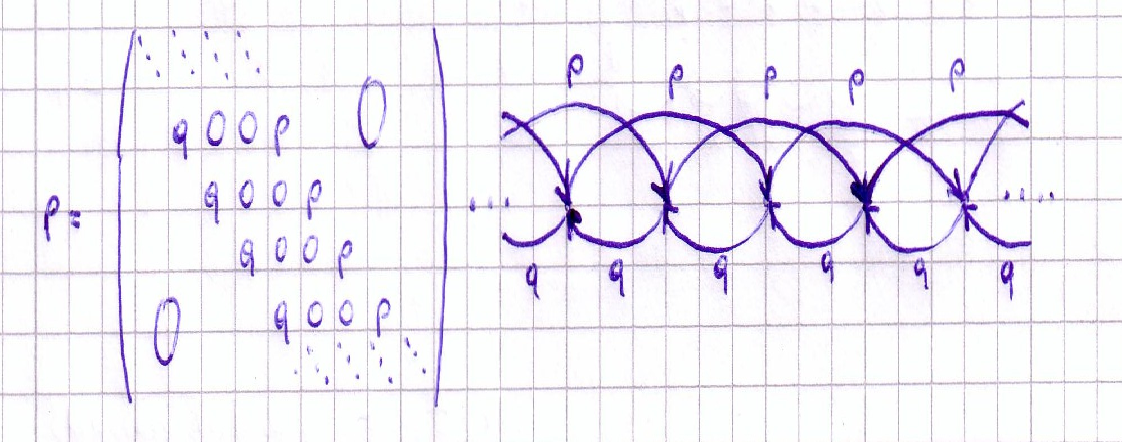
\includegraphics[width=14.825cm,height=3.706cm]{chapters/markovketten/a51Rekkurenz-img1.pdf}
\end{center}

%\bigskip


%\bigskip


%\bigskip


%\bigskip


%\bigskip


%\bigskip


%\bigskip


%\bigskip

{\selectlanguage{english}
Eine Bedingung f\"ur die Rekurrenz, die man praktisch ganz gut verwenden
kann, lautet:}


%\bigskip

\begin{equation*}
\sum _{t}p_{\mathit{ii}}(t)=\infty \text{    }(t\ge 1)
\end{equation*}

%\bigskip

{\selectlanguage{english}
 $p_{\mathit{ii}}(t)$ ist dabei nichts anderes als die
Wahrscheinlichkeit, \ in t Schritten (/Zeiten) von i nach i zu
gelangen. Da die Rekkurenz ja eine Klasseneigenschaft ist, w\"are es
egal welchen Zustand wir hier betrachten -- so k\"onnten wir 
$p_{00}(t)$ oder $p_{33}(t)$ oder sonst einen Zustand betrachten. Wir
betrachten hier (da wir die Zust\"anden nicht explizit benannt haben)
einen beliebigen Zustand i. Die \"Ubergangswahrscheinlichkeiten sind
hier eh bei jedem Zustand gleich.}


%\bigskip

{\selectlanguage{english}
Sehen wir uns einfach mal die ersten paar Glieder der Folge 
$p_{\mathit{ii}}(t)$  an. (Die Reihe bestimmen wir sp\"ater). Wir
versuchen Einfach Wege in unserem Graphen zu finden die uns von i nach
i f\"uhren und z\"ahlen dabei die Schritte.}


%\bigskip

\begin{equation*}
p_{\mathit{ii}}(1)=0
\end{equation*}
Da wir nicht in einem Schritt von unserem
Zustand wieder in unseren Zustand gelangen k\"onnen.
\begin{equation*}
p_{\mathit{ii}}(2)=0\text{ auch hier finden wir keinen Weg}
\end{equation*}
\begin{equation*}
p_{\mathit{ii}}(3)=?
\end{equation*}

%\bigskip

{\selectlanguage{english}
In 3 Schritten k\"onnen wir von i nach i gelangen. Aber daf\"ur gibt es
mehr als eine M\"oglichkeit. Denn wir k\"onnen die Permutationen von 
$\{\uparrow ,\downarrow ,\downarrow \}$ bilden. Genauer handelt es sich
hier um die Permutation einer Multimenge und wir berechnen:}


%\bigskip

\begin{equation*}
\frac{3!}{1!2!}=3=\left(\begin{matrix}3\\2\end{matrix}\right)
\end{equation*}
\begin{equation*}
p_{\mathit{ii}}(3)=\left(\begin{matrix}3\\2\end{matrix}\right)\cdot
p^{1}\cdot (1-p)^{2}
\end{equation*}

%\bigskip

\begin{equation*}
p_{\mathit{ii}}(4)=0\text{  wieder kein Weg zu finden!}
\end{equation*}

%\bigskip

\begin{equation*}
p_{\mathit{ii}}(5)=0\text{  wieder kein Weg zu finden!}
\end{equation*}

%\bigskip

\begin{equation*}
p_{\mathit{ii}}(6)=?
\end{equation*}

%\bigskip

{\selectlanguage{english}
Diesmal  $\{\uparrow ,\uparrow ,\downarrow ,\downarrow ,\downarrow
,\downarrow \}$ mit 
$\frac{6!}{2!4!}=15=\left(\begin{matrix}6\\2\end{matrix}\right)$ }


%\bigskip

\begin{equation*}
p_{\mathit{ii}}(6)=\left(\begin{matrix}6\\2\end{matrix}\right)p^{2}\cdot
(1-p)^{4}
\end{equation*}

%\bigskip

{\selectlanguage{english}
Wir k\"onnen die Vermutung aufstellen, dass es so weiter geht. }


%\bigskip

{\selectlanguage{english}
Demnach w\"are:}


%\bigskip

\begin{equation*}
p_{\mathit{ii}}(t)=\left\{\begin{matrix}\text{ 
}3|t\text{:}\left(\begin{matrix}t\\\frac{t}{3}\end{matrix}\right)\cdot
p^{\frac{t}{3}}\cdot (1-p)^{\frac{2t}{3}}\\3\nmid t\text{:  
}0\end{matrix}\right.
\end{equation*}
{\selectlanguage{english}
Wir wollen nun also zeigen, dass:}


%\bigskip

\begin{equation*}
\sum _{t}p_{\mathit{ii}}(t)=\infty \text{    }(t\ge 1)
\end{equation*}

%\bigskip

{\selectlanguage{english}
Wir setzen  $t=3k$ und berechnen:}


%\bigskip

\begin{equation*}
\sum _{k>0}\left(\begin{matrix}3k\\k\end{matrix}\right)\cdot p^{k}\cdot
(1-p)^{2k}=\frac{(3k)!}{k!\cdot (2k)!}\cdot p^{k}\cdot (1-p)^{2k}
\end{equation*}
{\selectlanguage{english}
Was hier hilfreich ist (auch wenn es im ersten Moment vl. \ nicht so
aussieht) ist die Stirling-Formel:}


%\bigskip

\begin{equation*}
n!\simeq \sqrt{2\pi n}\cdot (\frac{n}{e})^{n},\text{   f\"ur
}n\rightarrow \infty 
\end{equation*}

%\bigskip

{\selectlanguage{english}
Ersetzen wir unsere Fakult\"aten durch die Alternativen der
Stirling-Formel, dann k\"urzt sich letztendlich viel Weg ung es bleibt
schlie{\ss}lich:}


%\bigskip

\begin{equation*}
\sum _{k>0}\sqrt{\frac{3}{4\pi k}}\cdot
\left(\frac{27}{4}\right)^{k}\cdot p^{k}\cdot
(1-p)^{2k}=\sqrt{\frac{3}{4\pi }}\cdot \sum
_{k>0}\sqrt{\frac{1}{k}}\cdot \left(\frac{27}{4}\right)^{k}\cdot
p^{k}\cdot (1-p)^{2k}
\end{equation*}
{\selectlanguage{english}
Was hilft uns das?}


%\bigskip

{\selectlanguage{english}
Wir wissen, dass}

\begin{equation*}
\sum _{k>0}{\frac{1}{\sqrt{k}}}=\infty 
\end{equation*}
{\selectlanguage{english}
Damit gilt auch  $\sum _{k>0}{\frac{1}{\sqrt{k}}}\cdot 1=\infty $ also
wenn:}

\begin{equation*}
\left(\frac{27}{4}\right)^{k}\cdot p^{k}\cdot (1-p)^{2k}\ge 1\rightarrow
(\left(\frac{27}{4}\right)\cdot p\cdot (1-p)^{2})^{k}\ge 1\rightarrow
\left(\frac{27}{4}\right)\cdot p\cdot (1-p)^{2}\ge 1
\end{equation*}

%\bigskip

{\selectlanguage{english}
ist die Kette sicher rekurrent!}


%\bigskip

{\selectlanguage{english}
Aus der L\"osung der resultierenden Ungleichung 
$p^{3}-2p^{2}+p-\frac{4}{27}\ge 0$ ergeben sich die L\"osungen:}


%\bigskip

{\selectlanguage{english}
 $p=\frac{1}{3}$ und  $p\ge \frac{4}{3}$  womit wir die eindeutige
L\"osung  $p=\frac{1}{3}$ gefunden haben, denn die Wahrscheinlichkeit
kann nie gr\"o{\ss}er 1 sein!}



%\end{document}
\end{uebsp}

% This file was converted to LaTeX by Writer2LaTeX ver. 1.0.2
% see http://writer2latex.sourceforge.net for more info
%\documentclass[a4paper]{article}
%\usepackage[ascii]{inputenc}
%\usepackage[T1]{fontenc}
%\usepackage[english,english]{babel}
%\usepackage{amsmath}
%\usepackage{amssymb,amsfonts,textcomp}
%\usepackage{color}
%\usepackage{array}
%\usepackage{hhline}
%\usepackage{hyperref}
%\hypersetup{pdftex, colorlinks=true, linkcolor=blue, citecolor=blue, filecolor=blue, urlcolor=blue, pdftitle=, pdfauthor=, pdfsubject=, pdfkeywords=}
%\usepackage[pdftex]{graphicx}
% Page layout (geometry)
%\setlength\voffset{-1in}
%\setlength\hoffset{-1in}
%\setlength\topmargin{2cm}
%\setlength\oddsidemargin{2cm}
%\setlength\textheight{25.7cm}
%\setlength\textwidth{17.001cm}
%\setlength\footskip{0.0cm}
%\setlength\headheight{0cm}
%\setlength\headsep{0cm}
% Footnote rule
%\setlength{\skip\footins}{0.119cm}
%\renewcommand\footnoterule{\vspace*{-0.018cm}\setlength\leftskip{0pt}\setlength\rightskip{0pt plus 1fil}\noindent\textcolor{black}{\rule{0.25\columnwidth}{0.018cm}}\vspace*{0.101cm}}
% Pages styles
%\makeatletter
%\newcommand\ps@Standard{
%  \renewcommand\@oddhead{}
%  \renewcommand\@evenhead{}
%  \renewcommand\@oddfoot{}
%  \renewcommand\@evenfoot{}
%  \renewcommand\thepage{\arabic{page}}
%}
%\makeatother
%\pagestyle{Standard}
%\title{}
%\author{}
%\date{2014-02-25T10:01:05.420000000}
%\begin{document}
\begin{uebsp}
{\centering\selectlanguage{english}\bfseries
Altes Beispiel 5.2
\par}


%\bigskip

{\selectlanguage{english}
Nun wollen wir noch feststellen ob die Markovkette aus 5.1 positiv- oder
nullrekurrent ist.}
\index{Nullrekurrent!Beispiel}
\index{positiv Rekurrent!Beispiel}\\

\begin{center}\textbf{Lösung zu Übung 5.2}\end{center}

{\selectlanguage{english}
Wir wissen:}


%\bigskip

{\selectlanguage{english}
Wenn eine station\"are Verteilung f\"ur die Markovkette existiert, dann
ist die Markovkette positiv rekurrent, ansonsten nullrekurrent.}


%\bigskip

{\selectlanguage{english}
Also versuchen wir eine station\"are Verteilung zu berechnen, d.h.: wir
berechnen:}


%\bigskip

{\selectlanguage{english}
 $\pi _{j}=\sum _{i}\pi _{i}p_{\mathit{ij}}$ was gelichbedeutend ist
mit:  $\underline{{\pi }}\cdot P=\underline{{\pi }}$ (vgl.
Matrizenmultiplikation)}


%\bigskip

{\selectlanguage{english}
wobei  $\pi _{j}\text{ (bzw. }\pi _{i}\text{)}$ die Eintr\"age des
Wahrscheinlichkeitsvektors  $\underline{{\pi }}$ sind, welcher als
Zeilenvektor aufgefasst wird und .  $\pi _{j}$ Beschreibt also die
Wahrscheinlichkeit daf\"ur, dass sich die Kette in in Zustand j
aufh\"alt. Im Falle einer station\"aren Verteilung ist diese ja auch
vom Zeitpunkt unabh\"angig.}


%\bigskip

{\selectlanguage{english}
Wir schauen wiedermal als erstes auf unsere  $p_{\mathit{ij}}$ denn von
denen wissen wir, dass sie oft 0 sind.}


%\bigskip

{\selectlanguage{english}
So bleibt uns  $\pi _{j}=\pi _{i-2}\cdot p+\pi _{i+1}(1-p)$ f\"ur p
eingesetzt ergibt das:}


%\bigskip

\begin{equation*}
\pi _{j}=\frac{1}{3}\pi _{i-2}\cdot +{\frac{2}{3}}\cdot \pi _{i+1}
\end{equation*}
\begin{equation*}
2\pi _{i+1}-3\pi _{i}+\pi _{i-2}=0
\end{equation*}

%\bigskip


%\bigskip

{\selectlanguage{english}
So erhalten wir mit  $2z^{3}-3z^{2}+1=0$:  $z_{1}=1\text{ durch
probieren}$ und dann f\"ur  $2z^{2}-z-1=0$ :  $z_{2}=1\text{ und
}z_{3}=-{\frac{1}{2}}$ }


%\bigskip

{\selectlanguage{english}
Das wiederum f\"uhrt uns zur L\"osung:}

\begin{equation*}
\pi _{i}=(C_{1}+C_{2}i)z_{1,2}^{i}+C_{3}z_{3}^{i}
\end{equation*}
\begin{equation*}
\pi _{i}=C_{1}+iC_{2}+(-{\frac{1}{2}})^{i}C_{3}
\end{equation*}

%\bigskip

{\selectlanguage{english}
Unsere Zustandsmenge ist prinzipiell \"uber  $\mathbb{Z}$
identifizierbar. Das bedeutet aber auch, dass es Zust\"ande mit einer
''ID'' i gibt die gegen unendlich geht.
Bilden wir also f\"ur i den Grenzwert gegen  $\pm \infty $ wo es
schlie{\ss}lich auch Zust\"ande gibt, so stellen wir fest:}


%\bigskip

\begin{equation*}
\pi _{i}=C_{1}+\underbrace{iC_{2}}_{\rightarrow \pm \infty
}+\underbrace{(-{\frac{1}{2}})^{i}C_{3}}_{\rightarrow 0}
\end{equation*}
{\selectlanguage{english}
Da aber f\"ur die station\"are Verteilung aber gelten muss:  $\sum
_{i}\pi _{i}=1$ ,ergibt sich ein Widerspruch, d.h.: es existiert keine
station\"are Verteilung. Somit ist die Markovkette nullrekurrent.}


%\bigskip


%\bigskip


%\bigskip
%\end{document}
\end{uebsp}

% This file was converted to LaTeX by Writer2LaTeX ver. 1.0.2
% see http://writer2latex.sourceforge.net for more info
%\documentclass[a4paper]{article}
%\usepackage[ascii]{inputenc}
%\usepackage[T1]{fontenc}
%\usepackage[english,ngerman]{babel}
%\usepackage{amsmath}
%\usepackage{amssymb,amsfonts,textcomp}
%\usepackage{color}
%\usepackage{array}
%\usepackage{hhline}
%\usepackage{hyperref}
%\hypersetup{pdftex, colorlinks=true, linkcolor=blue, citecolor=blue, filecolor=blue, urlcolor=blue, pdftitle=, pdfauthor=, pdfsubject=, pdfkeywords=}
% Page layout (geometry)
%\setlength\voffset{-1in}
%\setlength\hoffset{-1in}
%\setlength\topmargin{2cm}
%\setlength\oddsidemargin{2cm}
%\setlength\textheight{25.7cm}
%\setlength\textwidth{17.001cm}
%\setlength\footskip{0.0cm}
%\setlength\headheight{0cm}
%\setlength\headsep{0cm}
% Footnote rule
%\setlength{\skip\footins}{0.119cm}
%\renewcommand\footnoterule{\vspace*{-0.018cm}\setlength\leftskip{0pt}\setlength\rightskip{0pt plus 1fil}\noindent\textcolor{black}{\rule{0.25\columnwidth}{0.018cm}}\vspace*{0.101cm}}
% Pages styles
%\makeatletter
%\newcommand\ps@Standard{
%  \renewcommand\@oddhead{}
%  \renewcommand\@evenhead{}
%  \renewcommand\@oddfoot{}
%  \renewcommand\@evenfoot{}
%  \renewcommand\thepage{\arabic{page}}
%}
%\makeatother
%\pagestyle{Standard}
%\title{}
%\author{}
%\date{2014-02-25T10:01:15.251000000}
%\begin{document}
\begin{uebsp}

{\centering\bfseries
Altes Beispiel 5.5
\par}


%\bigskip
\index{mittlere Absorptionszeit!Beispiel}
Um die mittlere Zeit bis zur Absorption einmal praktisch zu berechnen
kehren wir zur\"uck zu unserem Beispiel 4.1. \ Unsere absorbierenden
Zust\"ande sind hier: \{0\}: {\quotedblbase}Spieler A hat kein Kapital
mehr und verloren{\textquotedblleft} \ und \{a+b\}:
{\quotedblbase}Spieler A hat alles und gewonnen{\textquotedblleft}.\\


\begin{center}\textbf{Lösung zu Übung 5.5}\end{center}

%\bigskip

Somit wissen wir bereits:  $m_{0}=0$ und  $m_{a+b}=0$ 


%\bigskip

F\"ur unsere anderen Zust\"ande gilt: 

\begin{equation*}
m_{i}=1+\sum _{j}p_{\mathit{ij}}m_{j}
\end{equation*}

%\bigskip

Wenn das Summenzeichen im ersten Moment auch etwas abschreckend wirkt,
wird sich gleich herausstellen, dass es halb so schlimm ist, da ohnehin
die meisten  $p_{\mathit{ij}}=0$ sind. \ Denn von unserem Zustand i
gelangen wir nur zu den beiden Nachbarzust\"anden i-1 und i+1 und das
jeweils mit einer Wahrscheinlichkeit von  $\frac{1}{2}$ . D.h.: 
$m_{i}=1+\frac{1}{2}m_{i-1}+\frac{1}{2}m_{i+1}$


%\bigskip

Sehen wir uns nun an wie die Folge der  $m_{i}$ verl\"auft. 


%\bigskip


%\bigskip

\begin{equation*}
m_{1}=1+\frac{1}{2}m_{0}+\frac{1}{2}m_{2}=1+0+\frac{1}{2}m_{2}=1+\frac{1}{2}m_{2}
\end{equation*}

%\bigskip

\begin{equation*}
\rightarrow m_{2}=2m_{1}-2=2(m_{1}-1)
\end{equation*}

%\bigskip

 $m_{2}=1+\frac{1}{2}m_{1}+\frac{1}{2}m_{3}$  daraus folgt: 
$m_{3}=2m_{2}-2-m_{1}$ setzen wir nun f\"ur  $m_{2}$ den oben
erhaltenen Ausdruck ein, erhalten wir:


%\bigskip


\bigskip

\begin{equation*}
m_{3}=2(2(m_{1}-1))-2-m_{1}=4m_{1}-4-2-m_{1}=3m_{1}-6=3(m_{1}-2)
\end{equation*}
Wir k\"onnen also folgende Vermutung aufstellen:


%\bigskip


%\bigskip

\begin{equation*}
m_{i}=i(m_{1}-(i-1))=i(m_{1}+1-i)
\end{equation*}
Nun w\"are es noch sch\"on zu erfahren wie gro{\ss}  $m_{1}$ konkret
ist. Dies k\"onnen wir auch berechnen, da wir \ wissen, dass
$m_{a+b}=0$.


%\bigskip


%\bigskip

\begin{equation*}
m_{a+b}=(a+b)(m_{1}+1-(a+b))=(a+b)(m_{1}+1-a-b)=0
\end{equation*}
Wir k\"onnen davon ausgehen, dass  $(a+b)$ gr\"o{\ss}er 0 ist. Damit der
Ausdruck oben also 0 wird, muss  $(m_{1}+1-a-b)=0$ sein.


%\bigskip

So erhalten wir: 


%\bigskip

\begin{equation*}
m_{1}=a+b-1
\end{equation*}

\bigskip

Damit k\"onnen wir die mittlere Absorptionszeit berechnen f\"ur den
Fall, dass wir in Zustand a (so viel Kapital hat Spieler A zu beginn)
starten.


\bigskip

\begin{equation*}
m_{a}=a(m_{1}-(a-1))=a(a+b-1-a+1)=a(b)=\mathit{ab}
\end{equation*}
\begin{equation*}
m_{b}=b(m_{1}-(b-1))=b(a+b-1-b+1)=b(a)=\mathit{ab}
\end{equation*}

%\bigskip

%\end{document}
\end{uebsp}

\newExercPage
\setcounter{Exercise}{5}
% This file was converted to LaTeX by Writer2LaTeX ver. 1.0.2
% see http://writer2latex.sourceforge.net for more info
%\documentclass[a4paper]{article}
%\usepackage[ascii]{inputenc}
%\usepackage[T1]{fontenc}
%\usepackage[english,ngerman]{babel}
%%\usepackage{amsmath}
%\usepackage{amssymb,amsfonts,textcomp}
%\usepackage{color}
%\usepackage{array}
%\usepackage{hhline}
%\usepackage{hyperref}
%\hypersetup{pdftex, colorlinks=true, linkcolor=blue, citecolor=blue, filecolor=blue, urlcolor=blue, pdftitle=, pdfauthor=, pdfsubject=, pdfkeywords=}
% Text styles
%\newcommand\textstyleAbsatzStandardschriftart[1]{#1}
% Page layout (geometry)
%\setlength\voffset{-1in}
%\setlength\hoffset{-1in}
%\setlength\topmargin{2cm}
%\setlength\oddsidemargin{2cm}
%%\setlength\textheight{23.698002cm}
%\setlength\textwidth{17.001cm}
%\setlength\footskip{0.751cm}
%\setlength\headheight{1.251cm}
%\setlength\headsep{0cm}
% Footnote rule
%\setlength{\skip\footins}{0.119cm}
%\renewcommand\footnoterule{\vspace*{-0.018cm}\setlength\leftskip{0pt}\setlength\rightskip{0pt plus 1fil}\noindent\textcolor{black}{\rule{0.25\columnwidth}{0.018cm}}\vspace*{0.101cm}}
% Pages styles
%\makeatletter
%\newcommand\ps@MP{
%  \renewcommand\@oddhead{\"Ubung 5\hfill \hfill 27.11.2013}
%%  \renewcommand\@evenhead{\@oddhead}
%  \renewcommand\@oddfoot{Wahrscheinlichkeitsrechnung\hfill Markus Kessler\hfill Seite %\textstyleAbsatzStandardschriftart{\textbf{\thepage{}}} von %\textstyleAbsatzStandardschriftart{\textbf{?}} \textstyleAbsatzStandardschriftart{und %stochastische Prozesse}}
%%  \renewcommand\@evenfoot{\@oddfoot}
%%  \renewcommand\thepage{\arabic{page}}
%}
%\newcommand\ps@Standard{
%  \renewcommand\@oddhead{}
%  \renewcommand\@evenhead{}
%  \renewcommand\@oddfoot{}
%  \renewcommand\@evenfoot{}
%  \renewcommand\thepage{\arabic{page}}
%}
%\makeatother
%\pagestyle{Standard}
%\newcommand\normalsubformula[1]{\text{\mathversion{normal}$#1$}}
%\title{}
%\author{}
%\date{2014-02-25T11:16:06.549000000}
%\begin{document}
{
\newcommand\textstyleAbsatzStandardschriftart[1]{#1}
\newcommand\normalsubformula[1]{\text{\mathversion{normal}$#1$}}

\begin{uebsp}
\begin{Exercise}

{\selectlanguage{ngerman}\bfseries
In zwei Urnen befinden sich insgesamt N Kugeln. Es wird jeweils eine
Kugel zuf\"allig (gleichverteilt) ausgew\"ahlt und in die andere Urne
gelegt. Die Anzahl 
$\normalsubformula{\text{X}}_{\normalsubformula{\text{t}}}\normalsubformula{\text{~}}$
\textstyleAbsatzStandardschriftart{der Kugeln in Urne 1 nach t
Schritten bildet eine Markovkette. Bestimmen Sie Ihre \"Ubergangsmatrix
und die station\"are Verteilung.}}
\index{"Ubergangsmatrix@Übergangsmatrix!Beispiel}
\index{stationäre Verteilung!Beispiel}

\end{Exercise}
\begin{Answer}

%\bigskip


%\bigskip


%\bigskip


%\bigskip


%\bigskip

{\selectlanguage{ngerman}
F\"ur die \"Ubergangsmatrix werden die Wahrscheinlichkeiten in
Abh\"angigkeit der Gesamtkugeln definiert.}

\begin{equation*}
\normalsubformula{\text{P}}=\left(\begin{matrix}\normalsubformula{\text{0}}&\normalsubformula{\text{1}}&\normalsubformula{\text{0}}&\cdots
&\cdots &\cdots
&\normalsubformula{\text{0}}\\\frac{\normalsubformula{\text{1}}}{\normalsubformula{\text{N}}}&\normalsubformula{\text{0}}&\frac{\normalsubformula{\text{N}}-\normalsubformula{\text{1}}}{\normalsubformula{\text{N}}}&\normalsubformula{\text{0}}&\cdots
&\cdots
&\normalsubformula{\text{0}}\\\normalsubformula{\text{0}}&\frac{\normalsubformula{\text{2}}}{\normalsubformula{\text{N}}}&\normalsubformula{\text{0}}&\frac{\normalsubformula{\text{N}}-\normalsubformula{\text{2}}}{\normalsubformula{\text{N}}}&\normalsubformula{\text{0}}&\cdots
&\normalsubformula{\text{0}}\\\vdots &\ddots &\ddots &\ddots &\ddots
&\ddots &\vdots \\\normalsubformula{\text{0}}&\ddots &\ddots
&\normalsubformula{\text{0}}&\frac{\normalsubformula{\text{N}}-\normalsubformula{\text{1}}}{\normalsubformula{\text{N}}}&\normalsubformula{\text{0}}&\frac{\normalsubformula{\text{1}}}{\normalsubformula{\text{N}}}\\\normalsubformula{\text{0}}&\cdots
&\cdots &\cdots
&\normalsubformula{\text{0}}&\normalsubformula{\text{1}}&\normalsubformula{\text{0}}\end{matrix}\right)
\end{equation*}
\textstyleAbsatzStandardschriftart{\foreignlanguage{ngerman}{Wir bauen
uns nun rekursiv eine Formel f\"ur }} $\normalsubformula{\text{$\pi
$}}_{\normalsubformula{\text{i}}}\normalsubformula{\text{~}}$
\textstyleAbsatzStandardschriftart{\foreignlanguage{ngerman}{auf. Dabei
gibt i die Anzahl der Kugeln in Urne 1 an.}}

Wir versuchen nun im folgenden, $\pi_i$ als Funktion von $\pi_0$ darzustellen:
Beginnen wir bei $\pi_0$: diese kann nur von $\pi_1$ erreicht werden:
\[\pi_0=\frac{1}{N}\pi_1\;\;\Rightarrow\;\;\pi_1=N\cdot \pi_0\]

$\pi_1$ lässt sich nun darstellen als:
\[\pi_1=1\cdot\pi_0+\frac{2}{N}\cdot\pi_2\;\;\Rightarrow\;\;
N\cdot\pi_0-\pi_0=\frac{2}{N}\cdot\pi_2\;\;\Rightarrow\;\;
\pi_2=\frac{N(N-1)}{2}\pi_0\]

$\pi_2$ lässt sich nun darstellen als:
\[\pi_2=\frac{N-1}{N}\pi_1+\frac{3}{N}\pi_3\;\;\Rightarrow\;\;\frac{N(N-1)}{2}\pi_0=\frac{N-1}{\cancel N}\cancel N\cdot \pi_0+\frac{3}{N}\pi_3\;\;\Rightarrow\;\;\]
\[\frac{N(N-1)-2\cdot (N-1)}{2}\cdot \pi_0=\frac{3}{N}\pi_3\;\;\Rightarrow\;\;\pi_3=\frac{(N-2)(N-1)N}{2\cdot 3}\cdot \pi_0\]

\textstyleAbsatzStandardschriftart{\foreignlanguage{ngerman}{F\"ur }}
$\normalsubformula{\text{$\pi
$}}_{\normalsubformula{\text{i}}}\normalsubformula{\text{~}}$
\textstyleAbsatzStandardschriftart{\foreignlanguage{ngerman}{ergibt
das:}}

\begin{equation*}
\normalsubformula{\text{$\pi
$}}_{\normalsubformula{\text{i}}}=\frac{\normalsubformula{\text{N}}\left(\normalsubformula{\text{N}}-\normalsubformula{\text{1}}\right)\left(\normalsubformula{\text{N}}-\normalsubformula{\text{2}}\right)\ldots
\left(\normalsubformula{\text{N}}-\left(\normalsubformula{\text{i}}-\normalsubformula{\text{1}}\right)\right)}{\normalsubformula{\text{i}}!}\normalsubformula{\text{$\pi
$}}_{\normalsubformula{\text{0}}}
\end{equation*}
{\selectlanguage{ngerman}
Die Analogie zum Binomialkoeffizient:}

\begin{equation*}
\left(\begin{matrix}\normalsubformula{\text{n}}\\\normalsubformula{\text{k}}\end{matrix}\right)=\frac{\normalsubformula{\text{n}}!}{\normalsubformula{\text{k}}!\left(\normalsubformula{\text{n}}-\normalsubformula{\text{k}}\right)!}=\frac{\normalsubformula{\text{n}}\left(\normalsubformula{\text{n}}-\normalsubformula{\text{1}}\right)\left(\normalsubformula{\text{n}}-\normalsubformula{\text{2}}\right)\ldots
\left(\normalsubformula{\text{n}}-\left(\normalsubformula{\text{k}}-\normalsubformula{\text{1}}\right)\right)}{\normalsubformula{\text{k}}!}
\end{equation*}
\textstyleAbsatzStandardschriftart{\foreignlanguage{ngerman}{Wir
k\"onnen }} $\normalsubformula{\text{$\pi
$}}_{\normalsubformula{\text{i}}}\normalsubformula{\text{~}}$
\textstyleAbsatzStandardschriftart{\foreignlanguage{ngerman}{umschreiben:}}

\begin{equation*}
\normalsubformula{\text{$\pi
$}}_{\normalsubformula{\text{i}}}=\left(\begin{matrix}\normalsubformula{\text{N}}\\\normalsubformula{\text{i}}\end{matrix}\right)\normalsubformula{\text{$\pi
$}}_{\normalsubformula{\text{0}}}\normalsubformula{\text{~}}\normalsubformula{\text{~}}\normalsubformula{\text{~}}\normalsubformula{\text{~}}\normalsubformula{\text{~}}\normalsubformula{\text{m}}\normalsubformula{\text{i}}\normalsubformula{\text{t}}\normalsubformula{\text{~}}\normalsubformula{\text{i}}\in
[\normalsubformula{\text{0}},\normalsubformula{\text{N}}]
\end{equation*}
Die Summe \"uber alle  $\normalsubformula{\text{$\pi
$}}\normalsubformula{\text{~}}$
\textstyleAbsatzStandardschriftart{beinhaltet alle Wahrscheinlichkeiten
und muss 1 geben.}

\begin{equation*}
\sum
_{\normalsubformula{\text{i}}=\normalsubformula{\text{0}}}^{\normalsubformula{\text{N}}}\normalsubformula{\text{$\pi
$}}_{\normalsubformula{\text{i}}}=\normalsubformula{\text{1}}=\sum
_{\normalsubformula{\text{i}}=\normalsubformula{\text{0}}}^{\normalsubformula{\text{N}}}{\left(\begin{matrix}\normalsubformula{\text{N}}\\\normalsubformula{\text{i}}\end{matrix}\right)\normalsubformula{\text{$\pi
$}}_{\normalsubformula{\text{0}}}}=\normalsubformula{\text{$\pi
$}}_{\normalsubformula{\text{0}}}\sum
_{\normalsubformula{\text{i}}=\normalsubformula{\text{0}}}^{\normalsubformula{\text{N}}}\left(\begin{matrix}\normalsubformula{\text{N}}\\\normalsubformula{\text{i}}\end{matrix}\right)
\end{equation*}
Diese Summe k\"onnen wir durch den Binomischen Lehrsatz(siehe Anhang \ref{sec:binom_lehrsatz}) umschreiben:\index{Binomischer Lehrsatz!Beispiel}

\begin{equation*}
\normalsubformula{\text{$\pi $}}_{\normalsubformula{\text{0}}}\sum
_{\normalsubformula{\text{i}}=\normalsubformula{\text{0}}}^{\normalsubformula{\text{N}}}\left(\begin{matrix}\normalsubformula{\text{N}}\\\normalsubformula{\text{i}}\end{matrix}\right)=\normalsubformula{\text{$\pi
$}}_{\normalsubformula{\text{0}}}\sum
_{\normalsubformula{\text{i}}=\normalsubformula{\text{0}}}^{\normalsubformula{\text{N}}}{\left(\begin{matrix}\normalsubformula{\text{N}}\\\normalsubformula{\text{i}}\end{matrix}\right)\normalsubformula{\text{1}}^{\normalsubformula{\text{N}}-\normalsubformula{\text{1}}}\normalsubformula{\text{1}}^{\normalsubformula{\text{i}}}}=\normalsubformula{\text{$\pi
$}}_{\normalsubformula{\text{0}}}\left(\normalsubformula{\text{1}}+\normalsubformula{\text{1}}\right)^{\normalsubformula{\text{N}}}=\normalsubformula{\text{$\pi
$}}_{\normalsubformula{\text{0}}}\normalsubformula{\text{2}}^{\normalsubformula{\text{N}}}
\end{equation*}
{\selectlanguage{ngerman}
Wie bereits erw\"ahnt muss dies 1 ergeben:}

\begin{equation*}
\normalsubformula{\text{$\pi
$}}_{\normalsubformula{\text{0}}}\normalsubformula{\text{2}}^{\normalsubformula{\text{N}}}=\normalsubformula{\text{1}}\Rightarrow
\normalsubformula{\text{$\pi
$}}_{\normalsubformula{\text{0}}}=\frac{\normalsubformula{\text{1}}}{\normalsubformula{\text{2}}^{\normalsubformula{\text{N}}}}
\end{equation*}
\textstyleAbsatzStandardschriftart{\foreignlanguage{ngerman}{Eingesetzt
in }} $\normalsubformula{\text{$\pi
$}}_{\normalsubformula{\text{i}}}\normalsubformula{\text{~}}$
\textstyleAbsatzStandardschriftart{\foreignlanguage{ngerman}{erhalten
wir die station\"are Verteilung:}}

\begin{equation*}
\normalsubformula{\text{$\pi
$}}_{\normalsubformula{\text{i}}}=\left(\begin{matrix}\normalsubformula{\text{N}}\\\normalsubformula{\text{i}}\end{matrix}\right)\frac{\normalsubformula{\text{1}}}{\normalsubformula{\text{2}}^{\normalsubformula{\text{N}}}}
\end{equation*}
%\end{document}
\end{Answer}
\end{uebsp}
}

% This file was converted to LaTeX by Writer2LaTeX ver. 1.0.2
% see http://writer2latex.sourceforge.net for more info
%\documentclass[a4paper]{article}
%\usepackage[ascii]{inputenc}
%\usepackage[T1]{fontenc}
%\usepackage[english,ngerman]{babel}
%\usepackage{amsmath}
%\usepackage{amssymb,amsfonts,textcomp}
%\usepackage{color}
%\usepackage{array}
%\usepackage{hhline}
%\usepackage{hyperref}
%\hypersetup{pdftex, colorlinks=true, linkcolor=blue, citecolor=blue, filecolor=blue, urlcolor=blue, pdftitle=, pdfauthor=, pdfsubject=, pdfkeywords=}
% Text styles
%\newcommand\textstyleAbsatzStandardschriftart[1]{#1}
% Page layout (geometry)
%\setlength\voffset{-1in}
%\setlength\hoffset{-1in}
%\setlength\topmargin{2cm}
%\setlength\oddsidemargin{2cm}
%\setlength\textheight{23.698002cm}
%\setlength\textwidth{17.001cm}
%\setlength\footskip{0.751cm}
%%\setlength\headheight{1.251cm}
%\setlength\headsep{0cm}
% Footnote rule
%\setlength{\skip\footins}{0.119cm}
%\renewcommand\footnoterule{\vspace*{-0.018cm}\setlength\leftskip{0pt}\setlength\rightskip{0pt plus 1fil}\noindent\textcolor{black}{\rule{0.25\columnwidth}{0.018cm}}\vspace*{0.101cm}}
% Pages styles
%\makeatletter
%\newcommand\ps@MP{
%  \renewcommand\@oddhead{\"Ubung 5\hfill \hfill 27.11.2013}
%  \renewcommand\@evenhead{\@oddhead}
%  \renewcommand\@oddfoot{Wahrscheinlichkeitsrechnung\hfill Markus Kessler\hfill Seite %\textstyleAbsatzStandardschriftart{\textbf{\thepage{}}} von %\textstyleAbsatzStandardschriftart{\textbf{?}} \textstyleAbsatzStandardschriftart{und %stochastische Prozesse}}
%  \renewcommand\@evenfoot{\@oddfoot}
%  \renewcommand\thepage{\arabic{page}}
%}
%\newcommand\ps@Standard{
%  \renewcommand\@oddhead{}
%  \renewcommand\@evenhead{}
%  \renewcommand\@oddfoot{}
%  \renewcommand\@evenfoot{}
%  \renewcommand\thepage{\arabic{page}}
%}
%\makeatother
%\pagestyle{Standard}
%\newcommand\normalsubformula[1]{\text{\mathversion{normal}$#1$}}
%\title{}
%\author{}
%\date{2014-02-25T11:40:19.646000000}
%\begin{document}
%\clearpage\clearpage\setcounter{page}{1}\pagestyle{MP}
{
\begin{uebsp}
\newcommand\textstyleAbsatzStandardschriftart[1]{#1}
\newcommand\normalsubformula[1]{\text{\mathversion{normal}$#1$}}


%\bigskip

\begin{Exercise}
{\selectlanguage{ngerman}\bfseries
Die Markovkette 
$\normalsubformula{\text{X}}_{\normalsubformula{\text{t}}}\normalsubformula{\text{~}}$
\textstyleAbsatzStandardschriftart{mit Zustandsraum }
$\left(\normalsubformula{\text{0}},\ldots
,\normalsubformula{\text{N}}\right)\normalsubformula{\text{~}}$
\textstyleAbsatzStandardschriftart{hat die
\"Ubergangswahrscheinlichkeiten }\newline
\index{"Ubergangswahrscheinlichkeit@Übergangswahrscheinlichkeit!Beispiel}
\index{R"uckkehrzeit@Rückkehrzeit!Beispiel}

$\normalsubformula{\text{p}}_{\normalsubformula{\text{i}},\normalsubformula{\text{i}}+\normalsubformula{\text{1}}}=\normalsubformula{\text{p}}_{\normalsubformula{\text{i}}},\normalsubformula{\text{~}}\normalsubformula{\text{p}}_{\normalsubformula{\text{i}},\normalsubformula{\text{0}}}=\normalsubformula{\text{1}}-\normalsubformula{\text{p}}_{\normalsubformula{\text{i}}}\normalsubformula{\text{~}}$
\textstyleAbsatzStandardschriftart{mit }
$\normalsubformula{\text{p}}_{\normalsubformula{\text{N}}}=\normalsubformula{\text{0}}\text{.}\normalsubformula{\text{~}}$
\textstyleAbsatzStandardschriftart{Bestimmen Sie die Verteilung der
R\"uckkehrzeit } $\normalsubformula{\text{$\tau
$}}_{\normalsubformula{\text{0}}}\normalsubformula{\text{~}}$
\textstyleAbsatzStandardschriftart{nach 0. Wie muss man die }
$\normalsubformula{\text{p}}_{\normalsubformula{\text{i}}}\normalsubformula{\text{~}}$
\textstyleAbsatzStandardschriftart{w\"ahlen, damit }
$\normalsubformula{\text{t}}_{\normalsubformula{\text{i}}}\normalsubformula{\text{~}}$
\textstyleAbsatzStandardschriftart{auf }
$\left(\normalsubformula{\text{1}},\ldots
,\normalsubformula{\text{N}}+\normalsubformula{\text{1}}\right)\normalsubformula{\text{~}}$
\textstyleAbsatzStandardschriftart{gleichverteilt ist?}}
\end{Exercise}

\begin{Answer}
{\selectlanguage{ngerman}
Skizze}

{\selectlanguage{ngerman}
Die R\"uckkehrwahrscheinlichkeiten sind definiert mit:}

{\centering 
$\normalsubformula{\text{P}}\left(\normalsubformula{\text{$\tau
$}}_{\normalsubformula{\text{0}}}=\normalsubformula{\text{1}}\right)=\left(\normalsubformula{\text{1}}-\normalsubformula{\text{p}}_{\normalsubformula{\text{o}}}\right)$\newline
 $\normalsubformula{\text{P}}\left(\normalsubformula{\text{$\tau
$}}_{\normalsubformula{\text{0}}}=\normalsubformula{\text{2}}\right)=\normalsubformula{\text{p}}_{\normalsubformula{\text{0}}}\left(\normalsubformula{\text{1}}-\normalsubformula{\text{p}}_{\normalsubformula{\text{1}}}\right)$\newline
 $\normalsubformula{\text{P}}\left(\normalsubformula{\text{$\tau
$}}_{\normalsubformula{\text{0}}}=\normalsubformula{\text{3}}\right)=\normalsubformula{\text{p}}_{\normalsubformula{\text{0}}}\normalsubformula{\text{p}}_{\normalsubformula{\text{1}}}(\normalsubformula{\text{1}}-\normalsubformula{\text{p}}_{\normalsubformula{\text{2}}})$\par}

\textstyleAbsatzStandardschriftart{\foreignlanguage{ngerman}{Zur
Erkl\"arung: f\"ur }} $\normalsubformula{\text{$\tau
$}}_{\normalsubformula{\text{0}}}=\normalsubformula{\text{3}}\normalsubformula{\text{~}}$
\textstyleAbsatzStandardschriftart{\foreignlanguage{ngerman}{springe
ich nach drei Schritten zur\"uck zum Anfang. Daf\"ur kann ich nur den
Weg \"uber }}
$\normalsubformula{\text{p}}_{\normalsubformula{\text{0}}},\normalsubformula{\text{~}}{\normalsubformula{\text{~}}\normalsubformula{\text{p}}}_{\normalsubformula{\text{1}}}\normalsubformula{\text{~}}$
\textstyleAbsatzStandardschriftart{\foreignlanguage{ngerman}{und }}
$\left(\normalsubformula{\text{1}}-\normalsubformula{\text{p}}_{\normalsubformula{\text{2}}}\right)\normalsubformula{\text{~}}$
\textstyleAbsatzStandardschriftart{\foreignlanguage{ngerman}{gehen.}}

\begin{equation*}
\normalsubformula{\text{P}}\left(\normalsubformula{\text{$\tau
$}}_{\normalsubformula{\text{0}}}=\normalsubformula{\text{k}}\right)=\normalsubformula{\text{p}}_{\normalsubformula{\text{0}}}\normalsubformula{\text{p}}_{\normalsubformula{\text{1}}}\ldots
\normalsubformula{\text{P}}_{\normalsubformula{\text{k}}-\normalsubformula{\text{2}}}\left(\normalsubformula{\text{1}}-\normalsubformula{\text{p}}_{\normalsubformula{\text{k}}-\normalsubformula{\text{1}}}\right)\normalsubformula{\text{~}}\normalsubformula{\text{~}}\normalsubformula{\text{~}}\normalsubformula{\text{~}}\normalsubformula{\text{~}}\normalsubformula{\text{k}}\in
[\normalsubformula{\text{1}},\normalsubformula{\text{N}}+\normalsubformula{\text{1}}]
\end{equation*}
{\selectlanguage{ngerman}
Damit eine Gleichverteilung vorhanden ist, muss jede R\"uckkehrzeit
gleich wahrscheinlich sein.}

\begin{equation*}
\normalsubformula{\text{P}}\left(\normalsubformula{\text{$\tau
$}}_{\normalsubformula{\text{0}}}=\normalsubformula{\text{1}}\right)=\normalsubformula{\text{P}}\left(\normalsubformula{\text{$\tau
$}}_{\normalsubformula{\text{0}}}=\normalsubformula{\text{2}}\right)=\ldots
=\normalsubformula{\text{P}}\left(\normalsubformula{\text{$\tau
$}}_{\normalsubformula{\text{0}}}=\normalsubformula{\text{k}}\right)=\ldots
=\normalsubformula{\text{P}}(\normalsubformula{\text{$\tau
$}}_{\normalsubformula{\text{0}}}=\normalsubformula{\text{N}}+\normalsubformula{\text{1}})=\frac{\normalsubformula{\text{1}}}{\normalsubformula{\text{N}}+\normalsubformula{\text{1}}}
\end{equation*}
{\selectlanguage{ngerman}
Wir k\"onnen rekursiv beginnen:}

\begin{equation*}
\normalsubformula{\text{P}}(\normalsubformula{\text{$\tau
$}}_{\normalsubformula{\text{0}}}=\normalsubformula{\text{1}})
\end{equation*}
{\centering 
$\left(\normalsubformula{\text{1}}-\normalsubformula{\text{p}}_{\normalsubformula{\text{0}}}\right)=\frac{\normalsubformula{\text{1}}}{\normalsubformula{\text{N}}+\normalsubformula{\text{1}}}$\newline

$\normalsubformula{\text{p}}_{\normalsubformula{\text{0}}}=\normalsubformula{\text{1}}-\frac{\normalsubformula{\text{1}}}{\normalsubformula{\text{N}}+\normalsubformula{\text{1}}}=\frac{\normalsubformula{\text{N}}}{\normalsubformula{\text{N}}+\normalsubformula{\text{1}}}$\par}

\begin{equation*}
\normalsubformula{\text{P}}(\normalsubformula{\text{$\tau
$}}_{\normalsubformula{\text{0}}}=\normalsubformula{\text{2}})
\end{equation*}
{\centering 
$\normalsubformula{\text{p}}_{\normalsubformula{\text{0}}}\left(\normalsubformula{\text{1}}-\normalsubformula{\text{p}}_{\normalsubformula{\text{1}}}\right)=\frac{\normalsubformula{\text{1}}}{\normalsubformula{\text{N}}+\normalsubformula{\text{1}}}$\newline

$\frac{\normalsubformula{\text{N}}}{\normalsubformula{\text{N}}+\normalsubformula{\text{1}}}\left(\normalsubformula{\text{1}}-\normalsubformula{\text{p}}_{\normalsubformula{\text{1}}}\right)=\frac{\normalsubformula{\text{1}}}{\normalsubformula{\text{N}}+\normalsubformula{\text{1}}}$\newline

$\normalsubformula{\text{1}}-\normalsubformula{\text{p}}_{\normalsubformula{\text{1}}}=\frac{\normalsubformula{\text{1}}}{\normalsubformula{\text{N}}}$\newline

$\normalsubformula{\text{p}}_{\normalsubformula{\text{1}}}=\normalsubformula{\text{1}}-\frac{\normalsubformula{\text{1}}}{\normalsubformula{\text{N}}}=\frac{\normalsubformula{\text{N}}-\normalsubformula{\text{1}}}{\normalsubformula{\text{N}}}$\par}

\begin{equation*}
\normalsubformula{\text{P}}(\normalsubformula{\text{$\tau
$}}_{\normalsubformula{\text{0}}}=\normalsubformula{\text{3}})
\end{equation*}
{\centering 
$\normalsubformula{\text{p}}_{\normalsubformula{\text{0}}}\normalsubformula{\text{p}}_{\normalsubformula{\text{1}}}\left(\normalsubformula{\text{1}}-\normalsubformula{\text{p}}_{\normalsubformula{\text{2}}}\right)=\frac{\normalsubformula{\text{1}}}{\normalsubformula{\text{N}}+\normalsubformula{\text{1}}}$\newline

$\frac{\normalsubformula{\text{N}}}{\normalsubformula{\text{N}}+\normalsubformula{\text{1}}}\frac{\normalsubformula{\text{N}}-\normalsubformula{\text{1}}}{\normalsubformula{\text{N}}}\left(\normalsubformula{\text{1}}-\normalsubformula{\text{p}}_{\normalsubformula{\text{2}}}\right)=\frac{\normalsubformula{\text{1}}}{\normalsubformula{\text{N}}+\normalsubformula{\text{1}}}$\newline

$\normalsubformula{\text{1}}-\normalsubformula{\text{p}}_{\normalsubformula{\text{2}}}=\frac{\left(\normalsubformula{\text{N}}+\normalsubformula{\text{1}}\right)\normalsubformula{\text{N}}}{\left(\normalsubformula{\text{N}}+\normalsubformula{\text{1}}\right)\normalsubformula{\text{N}}\left(\normalsubformula{\text{N}}-\normalsubformula{\text{1}}\right)}=\frac{\normalsubformula{\text{1}}}{\normalsubformula{\text{N}}-\normalsubformula{\text{1}}}$\newline

$\normalsubformula{\text{p}}_{\normalsubformula{\text{2}}}=\normalsubformula{\text{1}}-\frac{\normalsubformula{\text{1}}}{\normalsubformula{\text{N}}-\normalsubformula{\text{1}}}=\frac{\normalsubformula{\text{N}}-\normalsubformula{\text{2}}}{\normalsubformula{\text{N}}-\normalsubformula{\text{1}}}$\par}

\textstyleAbsatzStandardschriftart{\foreignlanguage{ngerman}{F\"ur }}
$\normalsubformula{\text{p}}_{\normalsubformula{\text{k}}}\normalsubformula{\text{~}}$
\textstyleAbsatzStandardschriftart{\foreignlanguage{ngerman}{l\"asst
sich definieren:}}

\begin{equation*}
\normalsubformula{\text{p}}_{\normalsubformula{\text{k}}}=\frac{\normalsubformula{\text{N}}-\normalsubformula{\text{k}}}{\normalsubformula{\text{N}}-\normalsubformula{\text{k}}+\normalsubformula{\text{1}}}
\end{equation*}
\end{Answer}
\end{uebsp}
}

\newExercPage
\fi
